
% Default to the notebook output style

    


% Inherit from the specified cell style.




    
\documentclass[11pt,a4paper]{article}

    
    \usepackage[brazil]{babel}
    \usepackage[T1]{fontenc}
    % Nicer default font (+ math font) than Computer Modern for most use cases
    \usepackage{mathpazo}

    % Basic figure setup, for now with no caption control since it's done
    % automatically by Pandoc (which extracts ![](path) syntax from Markdown).
    \usepackage{graphicx}
    % We will generate all images so they have a width \maxwidth. This means
    % that they will get their normal width if they fit onto the page, but
    % are scaled down if they would overflow the margins.
    \makeatletter
    \def\maxwidth{\ifdim\Gin@nat@width>\linewidth\linewidth
    \else\Gin@nat@width\fi}
    \makeatother
    \let\Oldincludegraphics\includegraphics
    % Set max figure width to be 80% of text width, for now hardcoded.
    \renewcommand{\includegraphics}[1]{\Oldincludegraphics[width=.8\maxwidth]{#1}}
    % Ensure that by default, figures have no caption (until we provide a
    % proper Figure object with a Caption API and a way to capture that
    % in the conversion process - todo).
    \usepackage{caption}
    \DeclareCaptionLabelFormat{nolabel}{}
    \captionsetup{labelformat=nolabel}

    \usepackage{adjustbox} % Used to constrain images to a maximum size 
    \usepackage{xcolor} % Allow colors to be defined
    \usepackage{enumerate} % Needed for markdown enumerations to work
    \usepackage{geometry} % Used to adjust the document margins
    \usepackage{amsmath} % Equations
    \usepackage{amssymb} % Equations
    \usepackage{textcomp} % defines textquotesingle
    % Hack from http://tex.stackexchange.com/a/47451/13684:
    \AtBeginDocument{%
        \def\PYZsq{\textquotesingle}% Upright quotes in Pygmentized code
    }
    \usepackage{upquote} % Upright quotes for verbatim code
    \usepackage{eurosym} % defines \euro
    \usepackage[mathletters]{ucs} % Extended unicode (utf-8) support
    \usepackage[utf8x]{inputenc} % Allow utf-8 characters in the tex document
    \usepackage{fancyvrb} % verbatim replacement that allows latex
    \usepackage{grffile} % extends the file name processing of package graphics 
                         % to support a larger range 
    % The hyperref package gives us a pdf with properly built
    % internal navigation ('pdf bookmarks' for the table of contents,
    % internal cross-reference links, web links for URLs, etc.)
    \usepackage{hyperref}
    \usepackage{longtable} % longtable support required by pandoc >1.10
    \usepackage{booktabs}  % table support for pandoc > 1.12.2
    \usepackage[inline]{enumitem} % IRkernel/repr support (it uses the enumerate* environment)
    \usepackage[normalem]{ulem} % ulem is needed to support strikethroughs (\sout)
                                % normalem makes italics be italics, not underlines
    

    
    
    % Colors for the hyperref package
    \definecolor{urlcolor}{rgb}{0,.145,.698}
    \definecolor{linkcolor}{rgb}{.71,0.21,0.01}
    \definecolor{citecolor}{rgb}{.12,.54,.11}

    % ANSI colors
    \definecolor{ansi-black}{HTML}{3E424D}
    \definecolor{ansi-black-intense}{HTML}{282C36}
    \definecolor{ansi-red}{HTML}{E75C58}
    \definecolor{ansi-red-intense}{HTML}{B22B31}
    \definecolor{ansi-green}{HTML}{00A250}
    \definecolor{ansi-green-intense}{HTML}{007427}
    \definecolor{ansi-yellow}{HTML}{DDB62B}
    \definecolor{ansi-yellow-intense}{HTML}{B27D12}
    \definecolor{ansi-blue}{HTML}{208FFB}
    \definecolor{ansi-blue-intense}{HTML}{0065CA}
    \definecolor{ansi-magenta}{HTML}{D160C4}
    \definecolor{ansi-magenta-intense}{HTML}{A03196}
    \definecolor{ansi-cyan}{HTML}{60C6C8}
    \definecolor{ansi-cyan-intense}{HTML}{258F8F}
    \definecolor{ansi-white}{HTML}{C5C1B4}
    \definecolor{ansi-white-intense}{HTML}{A1A6B2}

    % commands and environments needed by pandoc snippets
    % extracted from the output of `pandoc -s`
    \providecommand{\tightlist}{%
      \setlength{\itemsep}{0pt}\setlength{\parskip}{0pt}}
    \DefineVerbatimEnvironment{Highlighting}{Verbatim}{commandchars=\\\{\}}
    % Add ',fontsize=\small' for more characters per line
    \newenvironment{Shaded}{}{}
    \newcommand{\KeywordTok}[1]{\textcolor[rgb]{0.00,0.44,0.13}{\textbf{{#1}}}}
    \newcommand{\DataTypeTok}[1]{\textcolor[rgb]{0.56,0.13,0.00}{{#1}}}
    \newcommand{\DecValTok}[1]{\textcolor[rgb]{0.25,0.63,0.44}{{#1}}}
    \newcommand{\BaseNTok}[1]{\textcolor[rgb]{0.25,0.63,0.44}{{#1}}}
    \newcommand{\FloatTok}[1]{\textcolor[rgb]{0.25,0.63,0.44}{{#1}}}
    \newcommand{\CharTok}[1]{\textcolor[rgb]{0.25,0.44,0.63}{{#1}}}
    \newcommand{\StringTok}[1]{\textcolor[rgb]{0.25,0.44,0.63}{{#1}}}
    \newcommand{\CommentTok}[1]{\textcolor[rgb]{0.38,0.63,0.69}{\textit{{#1}}}}
    \newcommand{\OtherTok}[1]{\textcolor[rgb]{0.00,0.44,0.13}{{#1}}}
    \newcommand{\AlertTok}[1]{\textcolor[rgb]{1.00,0.00,0.00}{\textbf{{#1}}}}
    \newcommand{\FunctionTok}[1]{\textcolor[rgb]{0.02,0.16,0.49}{{#1}}}
    \newcommand{\RegionMarkerTok}[1]{{#1}}
    \newcommand{\ErrorTok}[1]{\textcolor[rgb]{1.00,0.00,0.00}{\textbf{{#1}}}}
    \newcommand{\NormalTok}[1]{{#1}}
    
    % Additional commands for more recent versions of Pandoc
    \newcommand{\ConstantTok}[1]{\textcolor[rgb]{0.53,0.00,0.00}{{#1}}}
    \newcommand{\SpecialCharTok}[1]{\textcolor[rgb]{0.25,0.44,0.63}{{#1}}}
    \newcommand{\VerbatimStringTok}[1]{\textcolor[rgb]{0.25,0.44,0.63}{{#1}}}
    \newcommand{\SpecialStringTok}[1]{\textcolor[rgb]{0.73,0.40,0.53}{{#1}}}
    \newcommand{\ImportTok}[1]{{#1}}
    \newcommand{\DocumentationTok}[1]{\textcolor[rgb]{0.73,0.13,0.13}{\textit{{#1}}}}
    \newcommand{\AnnotationTok}[1]{\textcolor[rgb]{0.38,0.63,0.69}{\textbf{\textit{{#1}}}}}
    \newcommand{\CommentVarTok}[1]{\textcolor[rgb]{0.38,0.63,0.69}{\textbf{\textit{{#1}}}}}
    \newcommand{\VariableTok}[1]{\textcolor[rgb]{0.10,0.09,0.49}{{#1}}}
    \newcommand{\ControlFlowTok}[1]{\textcolor[rgb]{0.00,0.44,0.13}{\textbf{{#1}}}}
    \newcommand{\OperatorTok}[1]{\textcolor[rgb]{0.40,0.40,0.40}{{#1}}}
    \newcommand{\BuiltInTok}[1]{{#1}}
    \newcommand{\ExtensionTok}[1]{{#1}}
    \newcommand{\PreprocessorTok}[1]{\textcolor[rgb]{0.74,0.48,0.00}{{#1}}}
    \newcommand{\AttributeTok}[1]{\textcolor[rgb]{0.49,0.56,0.16}{{#1}}}
    \newcommand{\InformationTok}[1]{\textcolor[rgb]{0.38,0.63,0.69}{\textbf{\textit{{#1}}}}}
    \newcommand{\WarningTok}[1]{\textcolor[rgb]{0.38,0.63,0.69}{\textbf{\textit{{#1}}}}}
    
    
    % Define a nice break command that doesn't care if a line doesn't already
    % exist.
    \def\br{\hspace*{\fill} \\* }
    % Math Jax compatability definitions
    \def\gt{>}
    \def\lt{<}
    % Document parameters
    \title{Laços encaixados e uma introdução à sua otimização \\ 
           \small{MC102-2018s1-Aula10-180403}
           }
    \author{Arthur J. Catto, PhD \\
            \small{ajcatto@g.unicamp.br}
            }
    \date{05 de abril de 2018}

    % Pygments definitions
    
\makeatletter
\def\PY@reset{\let\PY@it=\relax \let\PY@bf=\relax%
    \let\PY@ul=\relax \let\PY@tc=\relax%
    \let\PY@bc=\relax \let\PY@ff=\relax}
\def\PY@tok#1{\csname PY@tok@#1\endcsname}
\def\PY@toks#1+{\ifx\relax#1\empty\else%
    \PY@tok{#1}\expandafter\PY@toks\fi}
\def\PY@do#1{\PY@bc{\PY@tc{\PY@ul{%
    \PY@it{\PY@bf{\PY@ff{#1}}}}}}}
\def\PY#1#2{\PY@reset\PY@toks#1+\relax+\PY@do{#2}}

\expandafter\def\csname PY@tok@w\endcsname{\def\PY@tc##1{\textcolor[rgb]{0.73,0.73,0.73}{##1}}}
\expandafter\def\csname PY@tok@c\endcsname{\let\PY@it=\textit\def\PY@tc##1{\textcolor[rgb]{0.25,0.50,0.50}{##1}}}
\expandafter\def\csname PY@tok@cp\endcsname{\def\PY@tc##1{\textcolor[rgb]{0.74,0.48,0.00}{##1}}}
\expandafter\def\csname PY@tok@k\endcsname{\let\PY@bf=\textbf\def\PY@tc##1{\textcolor[rgb]{0.00,0.50,0.00}{##1}}}
\expandafter\def\csname PY@tok@kp\endcsname{\def\PY@tc##1{\textcolor[rgb]{0.00,0.50,0.00}{##1}}}
\expandafter\def\csname PY@tok@kt\endcsname{\def\PY@tc##1{\textcolor[rgb]{0.69,0.00,0.25}{##1}}}
\expandafter\def\csname PY@tok@o\endcsname{\def\PY@tc##1{\textcolor[rgb]{0.40,0.40,0.40}{##1}}}
\expandafter\def\csname PY@tok@ow\endcsname{\let\PY@bf=\textbf\def\PY@tc##1{\textcolor[rgb]{0.67,0.13,1.00}{##1}}}
\expandafter\def\csname PY@tok@nb\endcsname{\def\PY@tc##1{\textcolor[rgb]{0.00,0.50,0.00}{##1}}}
\expandafter\def\csname PY@tok@nf\endcsname{\def\PY@tc##1{\textcolor[rgb]{0.00,0.00,1.00}{##1}}}
\expandafter\def\csname PY@tok@nc\endcsname{\let\PY@bf=\textbf\def\PY@tc##1{\textcolor[rgb]{0.00,0.00,1.00}{##1}}}
\expandafter\def\csname PY@tok@nn\endcsname{\let\PY@bf=\textbf\def\PY@tc##1{\textcolor[rgb]{0.00,0.00,1.00}{##1}}}
\expandafter\def\csname PY@tok@ne\endcsname{\let\PY@bf=\textbf\def\PY@tc##1{\textcolor[rgb]{0.82,0.25,0.23}{##1}}}
\expandafter\def\csname PY@tok@nv\endcsname{\def\PY@tc##1{\textcolor[rgb]{0.10,0.09,0.49}{##1}}}
\expandafter\def\csname PY@tok@no\endcsname{\def\PY@tc##1{\textcolor[rgb]{0.53,0.00,0.00}{##1}}}
\expandafter\def\csname PY@tok@nl\endcsname{\def\PY@tc##1{\textcolor[rgb]{0.63,0.63,0.00}{##1}}}
\expandafter\def\csname PY@tok@ni\endcsname{\let\PY@bf=\textbf\def\PY@tc##1{\textcolor[rgb]{0.60,0.60,0.60}{##1}}}
\expandafter\def\csname PY@tok@na\endcsname{\def\PY@tc##1{\textcolor[rgb]{0.49,0.56,0.16}{##1}}}
\expandafter\def\csname PY@tok@nt\endcsname{\let\PY@bf=\textbf\def\PY@tc##1{\textcolor[rgb]{0.00,0.50,0.00}{##1}}}
\expandafter\def\csname PY@tok@nd\endcsname{\def\PY@tc##1{\textcolor[rgb]{0.67,0.13,1.00}{##1}}}
\expandafter\def\csname PY@tok@s\endcsname{\def\PY@tc##1{\textcolor[rgb]{0.73,0.13,0.13}{##1}}}
\expandafter\def\csname PY@tok@sd\endcsname{\let\PY@it=\textit\def\PY@tc##1{\textcolor[rgb]{0.73,0.13,0.13}{##1}}}
\expandafter\def\csname PY@tok@si\endcsname{\let\PY@bf=\textbf\def\PY@tc##1{\textcolor[rgb]{0.73,0.40,0.53}{##1}}}
\expandafter\def\csname PY@tok@se\endcsname{\let\PY@bf=\textbf\def\PY@tc##1{\textcolor[rgb]{0.73,0.40,0.13}{##1}}}
\expandafter\def\csname PY@tok@sr\endcsname{\def\PY@tc##1{\textcolor[rgb]{0.73,0.40,0.53}{##1}}}
\expandafter\def\csname PY@tok@ss\endcsname{\def\PY@tc##1{\textcolor[rgb]{0.10,0.09,0.49}{##1}}}
\expandafter\def\csname PY@tok@sx\endcsname{\def\PY@tc##1{\textcolor[rgb]{0.00,0.50,0.00}{##1}}}
\expandafter\def\csname PY@tok@m\endcsname{\def\PY@tc##1{\textcolor[rgb]{0.40,0.40,0.40}{##1}}}
\expandafter\def\csname PY@tok@gh\endcsname{\let\PY@bf=\textbf\def\PY@tc##1{\textcolor[rgb]{0.00,0.00,0.50}{##1}}}
\expandafter\def\csname PY@tok@gu\endcsname{\let\PY@bf=\textbf\def\PY@tc##1{\textcolor[rgb]{0.50,0.00,0.50}{##1}}}
\expandafter\def\csname PY@tok@gd\endcsname{\def\PY@tc##1{\textcolor[rgb]{0.63,0.00,0.00}{##1}}}
\expandafter\def\csname PY@tok@gi\endcsname{\def\PY@tc##1{\textcolor[rgb]{0.00,0.63,0.00}{##1}}}
\expandafter\def\csname PY@tok@gr\endcsname{\def\PY@tc##1{\textcolor[rgb]{1.00,0.00,0.00}{##1}}}
\expandafter\def\csname PY@tok@ge\endcsname{\let\PY@it=\textit}
\expandafter\def\csname PY@tok@gs\endcsname{\let\PY@bf=\textbf}
\expandafter\def\csname PY@tok@gp\endcsname{\let\PY@bf=\textbf\def\PY@tc##1{\textcolor[rgb]{0.00,0.00,0.50}{##1}}}
\expandafter\def\csname PY@tok@go\endcsname{\def\PY@tc##1{\textcolor[rgb]{0.53,0.53,0.53}{##1}}}
\expandafter\def\csname PY@tok@gt\endcsname{\def\PY@tc##1{\textcolor[rgb]{0.00,0.27,0.87}{##1}}}
\expandafter\def\csname PY@tok@err\endcsname{\def\PY@bc##1{\setlength{\fboxsep}{0pt}\fcolorbox[rgb]{1.00,0.00,0.00}{1,1,1}{\strut ##1}}}
\expandafter\def\csname PY@tok@kc\endcsname{\let\PY@bf=\textbf\def\PY@tc##1{\textcolor[rgb]{0.00,0.50,0.00}{##1}}}
\expandafter\def\csname PY@tok@kd\endcsname{\let\PY@bf=\textbf\def\PY@tc##1{\textcolor[rgb]{0.00,0.50,0.00}{##1}}}
\expandafter\def\csname PY@tok@kn\endcsname{\let\PY@bf=\textbf\def\PY@tc##1{\textcolor[rgb]{0.00,0.50,0.00}{##1}}}
\expandafter\def\csname PY@tok@kr\endcsname{\let\PY@bf=\textbf\def\PY@tc##1{\textcolor[rgb]{0.00,0.50,0.00}{##1}}}
\expandafter\def\csname PY@tok@bp\endcsname{\def\PY@tc##1{\textcolor[rgb]{0.00,0.50,0.00}{##1}}}
\expandafter\def\csname PY@tok@fm\endcsname{\def\PY@tc##1{\textcolor[rgb]{0.00,0.00,1.00}{##1}}}
\expandafter\def\csname PY@tok@vc\endcsname{\def\PY@tc##1{\textcolor[rgb]{0.10,0.09,0.49}{##1}}}
\expandafter\def\csname PY@tok@vg\endcsname{\def\PY@tc##1{\textcolor[rgb]{0.10,0.09,0.49}{##1}}}
\expandafter\def\csname PY@tok@vi\endcsname{\def\PY@tc##1{\textcolor[rgb]{0.10,0.09,0.49}{##1}}}
\expandafter\def\csname PY@tok@vm\endcsname{\def\PY@tc##1{\textcolor[rgb]{0.10,0.09,0.49}{##1}}}
\expandafter\def\csname PY@tok@sa\endcsname{\def\PY@tc##1{\textcolor[rgb]{0.73,0.13,0.13}{##1}}}
\expandafter\def\csname PY@tok@sb\endcsname{\def\PY@tc##1{\textcolor[rgb]{0.73,0.13,0.13}{##1}}}
\expandafter\def\csname PY@tok@sc\endcsname{\def\PY@tc##1{\textcolor[rgb]{0.73,0.13,0.13}{##1}}}
\expandafter\def\csname PY@tok@dl\endcsname{\def\PY@tc##1{\textcolor[rgb]{0.73,0.13,0.13}{##1}}}
\expandafter\def\csname PY@tok@s2\endcsname{\def\PY@tc##1{\textcolor[rgb]{0.73,0.13,0.13}{##1}}}
\expandafter\def\csname PY@tok@sh\endcsname{\def\PY@tc##1{\textcolor[rgb]{0.73,0.13,0.13}{##1}}}
\expandafter\def\csname PY@tok@s1\endcsname{\def\PY@tc##1{\textcolor[rgb]{0.73,0.13,0.13}{##1}}}
\expandafter\def\csname PY@tok@mb\endcsname{\def\PY@tc##1{\textcolor[rgb]{0.40,0.40,0.40}{##1}}}
\expandafter\def\csname PY@tok@mf\endcsname{\def\PY@tc##1{\textcolor[rgb]{0.40,0.40,0.40}{##1}}}
\expandafter\def\csname PY@tok@mh\endcsname{\def\PY@tc##1{\textcolor[rgb]{0.40,0.40,0.40}{##1}}}
\expandafter\def\csname PY@tok@mi\endcsname{\def\PY@tc##1{\textcolor[rgb]{0.40,0.40,0.40}{##1}}}
\expandafter\def\csname PY@tok@il\endcsname{\def\PY@tc##1{\textcolor[rgb]{0.40,0.40,0.40}{##1}}}
\expandafter\def\csname PY@tok@mo\endcsname{\def\PY@tc##1{\textcolor[rgb]{0.40,0.40,0.40}{##1}}}
\expandafter\def\csname PY@tok@ch\endcsname{\let\PY@it=\textit\def\PY@tc##1{\textcolor[rgb]{0.25,0.50,0.50}{##1}}}
\expandafter\def\csname PY@tok@cm\endcsname{\let\PY@it=\textit\def\PY@tc##1{\textcolor[rgb]{0.25,0.50,0.50}{##1}}}
\expandafter\def\csname PY@tok@cpf\endcsname{\let\PY@it=\textit\def\PY@tc##1{\textcolor[rgb]{0.25,0.50,0.50}{##1}}}
\expandafter\def\csname PY@tok@c1\endcsname{\let\PY@it=\textit\def\PY@tc##1{\textcolor[rgb]{0.25,0.50,0.50}{##1}}}
\expandafter\def\csname PY@tok@cs\endcsname{\let\PY@it=\textit\def\PY@tc##1{\textcolor[rgb]{0.25,0.50,0.50}{##1}}}

\def\PYZbs{\char`\\}
\def\PYZus{\char`\_}
\def\PYZob{\char`\{}
\def\PYZcb{\char`\}}
\def\PYZca{\char`\^}
\def\PYZam{\char`\&}
\def\PYZlt{\char`\<}
\def\PYZgt{\char`\>}
\def\PYZsh{\char`\#}
\def\PYZpc{\char`\%}
\def\PYZdl{\char`\$}
\def\PYZhy{\char`\-}
\def\PYZsq{\char`\'}
\def\PYZdq{\char`\"}
\def\PYZti{\char`\~}
% for compatibility with earlier versions
\def\PYZat{@}
\def\PYZlb{[}
\def\PYZrb{]}
\makeatother


    % Exact colors from NB
    \definecolor{incolor}{rgb}{0.0, 0.0, 0.5}
    \definecolor{outcolor}{rgb}{0.545, 0.0, 0.0}



    
    % Prevent overflowing lines due to hard-to-break entities
    \sloppy 
    % Setup hyperref package
    \hypersetup{
      breaklinks=true,  % so long urls are correctly broken across lines
      colorlinks=true,
      urlcolor=urlcolor,
      linkcolor=linkcolor,
      citecolor=citecolor,
      }
    % Slightly bigger margins than the latex defaults
    
    \geometry{verbose,tmargin=1in,bmargin=1in,lmargin=1in,rmargin=1in}
    
    

    \begin{document}
    
    
    \maketitle
    
    

%    
%    \begin{Verbatim}[commandchars=\\\{\}]
%{\color{incolor}In [{\color{incolor}1}]:} \PY{k+kn}{from} \PY{n+nn}{IPython}\PY{n+nn}{.}\PY{n+nn}{core}\PY{n+nn}{.}\PY{n+nn}{interactiveshell} \PY{k}{import} \PY{n}{InteractiveShell}
%        \PY{n}{InteractiveShell}\PY{o}{.}\PY{n}{ast\PYZus{}node\PYZus{}interactivity} \PY{o}{=} \PY{l+s+s2}{\PYZdq{}}\PY{l+s+s2}{all}\PY{l+s+s2}{\PYZdq{}}
%\end{Verbatim}


    \section{Laços encaixados e uma introdução à sua
otimização}\label{lauxe7os-encaixados-e-uma-introduuxe7uxe3o-uxe0-sua-otimizauxe7uxe3o}

    \subsection{\texorpdfstring{Exemplo: \emph{Dada uma sequência arbitrária
de inteiros não-negativos, encontrar o par mais
próximo}}{Exemplo: Dada uma sequência arbitrária de inteiros não-negativos, encontrar o par mais próximo}}\label{exemplo-dada-uma-sequuxeancia-arbitruxe1ria-de-inteiros-nuxe3o-negativos-encontrar-o-par-mais-pruxf3ximo}

Ler uma sequência arbitrária \(S\) de \(n\) inteiros não-negativos e
\textbf{\emph{depois}} encontrar \(i, 0 \le i \lt n\) e
\(j, 0 \le j \lt n\), \(i \ne j\), tais que a distância entre \(S_i\) e
\(S_j\), isto é, \(\lvert S_i - S_j \rvert\), seja mínima.

    \subsubsection{Desenvolvimento da
solução}\label{desenvolvimento-da-soluuxe7uxe3o}

    Em nível mais abstrato, a solução deste problema tem estrutura
semelhante à de vários exemplos anteriores:

\begin{Shaded}
\begin{Highlighting}[]
\NormalTok{ler a sequência S}
\NormalTok{encontrar os dois elementos mais próximos em S}
\NormalTok{exibir a solução}
\end{Highlighting}
\end{Shaded}

    Para \texttt{“ler\ a\ sequência\ S”} temos pelo menos duas saídas já
conhecidas:

    \begin{Verbatim}[commandchars=\\\{\}]
{\color{incolor}In [{\color{incolor}2}]:} \PY{n}{n} \PY{o}{=} \PY{n+nb}{int}\PY{p}{(}\PY{n+nb}{input}\PY{p}{(}\PY{l+s+s1}{\PYZsq{}}\PY{l+s+s1}{Número de elementos? }\PY{l+s+s1}{\PYZsq{}}\PY{p}{)}\PY{p}{)}
        \PY{n}{S} \PY{o}{=} \PY{p}{[}\PY{p}{]}
        \PY{k}{for} \PY{n}{i} \PY{o+ow}{in} \PY{n+nb}{range}\PY{p}{(}\PY{n}{n}\PY{p}{)}\PY{p}{:}
            \PY{n}{S}\PY{o}{.}\PY{n}{append}\PY{p}{(}\PY{n+nb}{int}\PY{p}{(}\PY{n+nb}{input}\PY{p}{(}\PY{l+s+s1}{\PYZsq{}}\PY{l+s+s1}{Elemento \PYZsh{}}\PY{l+s+s1}{\PYZsq{}} \PY{o}{+} \PY{n+nb}{str}\PY{p}{(}\PY{n}{i} \PY{o}{+} \PY{l+m+mi}{1}\PY{p}{)} \PY{o}{+} \PY{l+s+s1}{\PYZsq{}}\PY{l+s+s1}{? }\PY{l+s+s1}{\PYZsq{}}\PY{p}{)}\PY{p}{)}\PY{p}{)}
        \PY{n+nb}{print}\PY{p}{(}\PY{n}{S}\PY{p}{)}
\end{Verbatim}


    \begin{Verbatim}[commandchars=\\\{\}]
[12, 23, 34, 45, 56]

    \end{Verbatim}

    \begin{Verbatim}[commandchars=\\\{\}]
{\color{incolor}In [{\color{incolor}3}]:} \PY{n}{S} \PY{o}{=} \PY{p}{[}\PY{n+nb}{int}\PY{p}{(}\PY{n}{x}\PY{p}{)} \PY{k}{for} \PY{n}{x} \PY{o+ow}{in} \PY{n+nb}{input}\PY{p}{(}\PY{l+s+s1}{\PYZsq{}}\PY{l+s+s1}{Sequência de inteiros? }\PY{l+s+s1}{\PYZsq{}}\PY{p}{)}\PY{o}{.}\PY{n}{split}\PY{p}{(}\PY{p}{)}\PY{p}{]}
        \PY{n+nb}{print}\PY{p}{(}\PY{n}{S}\PY{p}{)}
\end{Verbatim}


    \begin{Verbatim}[commandchars=\\\{\}]
[12, 23, 34, 45, 56]

    \end{Verbatim}

    No entanto, em problemas como este, em geral vamos querer trabalhar com
sequências mais longas.\\
Isso inviabiliza a digitação de valores, especialmente quando se lembra
que a execução poderá ter que ser repetida diversas vezes enquanto
depuramos o algoritmo.

Uma saída mais apropriada é gerar uma sequência de valores
psudo-aleatórios usando o módulo \emph{random}.

    \begin{Verbatim}[commandchars=\\\{\}]
{\color{incolor}In [{\color{incolor}4}]:} \PY{k+kn}{from} \PY{n+nn}{random} \PY{k}{import} \PY{n}{choices}
        
        \PY{n}{n} \PY{o}{=} \PY{l+m+mi}{10}
        \PY{n}{S} \PY{o}{=} \PY{n}{choices}\PY{p}{(}\PY{n+nb}{range}\PY{p}{(}\PY{l+m+mi}{1000000}\PY{p}{)}\PY{p}{,} \PY{n}{k}\PY{o}{=}\PY{n}{n}\PY{p}{)}
        \PY{n+nb}{print}\PY{p}{(}\PY{n}{S}\PY{p}{[}\PY{p}{:}\PY{l+m+mi}{10}\PY{p}{]}\PY{p}{)}
        \PY{n+nb}{print}\PY{p}{(}\PY{n}{S}\PY{p}{[}\PY{o}{\PYZhy{}}\PY{l+m+mi}{10}\PY{p}{:}\PY{p}{]}\PY{p}{)}
\end{Verbatim}


    \begin{Verbatim}[commandchars=\\\{\}]
[500815, 694131, 372196, 892086, 397934, 4934, 813883, 901277, 767670, 261677]
[500815, 694131, 372196, 892086, 397934, 4934, 813883, 901277, 767670, 261677]

    \end{Verbatim}

    Sequências de números pseudo-aleatórios são geradas a partir de uma
\emph{semente}. Se usarmos uma mesma \emph{semente} seremos capazes de
repetir uma sequência quantas vezes quisermos.

Para gerar uma sequência ``imprevisível'', em geral usamos o valor do
relógio da máquina como \emph{semente}.\\
Se salvarmos o valor usado como \emph{semente}, a sequência poderá ser
repetida. Por exemplo,...

    \begin{Verbatim}[commandchars=\\\{\}]
{\color{incolor}In [{\color{incolor}5}]:} \PY{k+kn}{import} \PY{n+nn}{time}
        \PY{k+kn}{import} \PY{n+nn}{random}
\end{Verbatim}


    \begin{Verbatim}[commandchars=\\\{\}]
{\color{incolor}In [{\color{incolor}6}]:} \PY{n}{t\PYZus{}inicial} \PY{o}{=} \PY{n}{time}\PY{o}{.}\PY{n}{time}\PY{p}{(}\PY{p}{)}
        \PY{n}{t\PYZus{}inicial}
\end{Verbatim}


\begin{Verbatim}[commandchars=\\\{\}]
{\color{outcolor}Out[{\color{outcolor}6}]:} 1522894266.992621
\end{Verbatim}
            
    \begin{Verbatim}[commandchars=\\\{\}]
{\color{incolor}In [{\color{incolor}7}]:} \PY{n}{random}\PY{o}{.}\PY{n}{seed}\PY{p}{(}\PY{n}{t\PYZus{}inicial}\PY{p}{)}
        
        \PY{n}{S1} \PY{o}{=} \PY{n}{random}\PY{o}{.}\PY{n}{choices}\PY{p}{(}\PY{n+nb}{range}\PY{p}{(}\PY{l+m+mi}{1000000}\PY{p}{)}\PY{p}{,} \PY{n}{k}\PY{o}{=}\PY{l+m+mi}{10}\PY{p}{)}
        \PY{n+nb}{print}\PY{p}{(}\PY{n}{S1}\PY{p}{)}
\end{Verbatim}


    \begin{Verbatim}[commandchars=\\\{\}]
[683022, 240020, 532725, 677507, 228121, 376049, 469446, 138107, 901865, 869104]

    \end{Verbatim}

    \begin{Verbatim}[commandchars=\\\{\}]
{\color{incolor}In [{\color{incolor}8}]:} \PY{n}{S2} \PY{o}{=} \PY{n}{random}\PY{o}{.}\PY{n}{choices}\PY{p}{(}\PY{n+nb}{range}\PY{p}{(}\PY{l+m+mi}{1000000}\PY{p}{)}\PY{p}{,} \PY{n}{k}\PY{o}{=}\PY{l+m+mi}{10}\PY{p}{)}
        \PY{n+nb}{print}\PY{p}{(}\PY{n}{S2}\PY{p}{)}
\end{Verbatim}


    \begin{Verbatim}[commandchars=\\\{\}]
[66377, 243989, 165177, 620341, 80404, 718506, 632689, 508072, 364610, 835636]

    \end{Verbatim}

    \begin{Verbatim}[commandchars=\\\{\}]
{\color{incolor}In [{\color{incolor}9}]:} \PY{n}{S1} \PY{o}{==} \PY{n}{S2}
\end{Verbatim}


\begin{Verbatim}[commandchars=\\\{\}]
{\color{outcolor}Out[{\color{outcolor}9}]:} False
\end{Verbatim}
            
    Neste caso, geramos \texttt{S1} e depois \texttt{S2}, sem ``re-semear''
o gerador de aleatórios. Por causa disso, \texttt{S1} e \texttt{S2} são
diferentes.

No entanto, quando ``re-semeamos'' o gerador, obtemos \texttt{S3} igual
a \texttt{S1}.

    \begin{Verbatim}[commandchars=\\\{\}]
{\color{incolor}In [{\color{incolor}10}]:} \PY{n}{random}\PY{o}{.}\PY{n}{seed}\PY{p}{(}\PY{n}{t\PYZus{}inicial}\PY{p}{)}
         
         \PY{n}{S3} \PY{o}{=} \PY{n}{random}\PY{o}{.}\PY{n}{choices}\PY{p}{(}\PY{n+nb}{range}\PY{p}{(}\PY{l+m+mi}{1000000}\PY{p}{)}\PY{p}{,} \PY{n}{k}\PY{o}{=}\PY{l+m+mi}{10}\PY{p}{)}
         \PY{n+nb}{print}\PY{p}{(}\PY{n}{S3}\PY{p}{)}
\end{Verbatim}


    \begin{Verbatim}[commandchars=\\\{\}]
[683022, 240020, 532725, 677507, 228121, 376049, 469446, 138107, 901865, 869104]

    \end{Verbatim}

    \begin{Verbatim}[commandchars=\\\{\}]
{\color{incolor}In [{\color{incolor}11}]:} \PY{n}{S1} \PY{o}{==} \PY{n}{S3}
\end{Verbatim}


\begin{Verbatim}[commandchars=\\\{\}]
{\color{outcolor}Out[{\color{outcolor}11}]:} True
\end{Verbatim}
            
    Com isso, nossa geração de dados fica assim...

    \begin{Verbatim}[commandchars=\\\{\}]
{\color{incolor}In [{\color{incolor}12}]:} \PY{k+kn}{import} \PY{n+nn}{time}
         \PY{k+kn}{import} \PY{n+nn}{random}
\end{Verbatim}


    \begin{Verbatim}[commandchars=\\\{\}]
{\color{incolor}In [{\color{incolor}13}]:} \PY{n}{t\PYZus{}inicial} \PY{o}{=} \PY{n}{time}\PY{o}{.}\PY{n}{time}\PY{p}{(}\PY{p}{)}
\end{Verbatim}


    \begin{Verbatim}[commandchars=\\\{\}]
{\color{incolor}In [{\color{incolor}14}]:} \PY{n}{random}\PY{o}{.}\PY{n}{seed}\PY{p}{(}\PY{n}{t\PYZus{}inicial}\PY{p}{)}
         
         \PY{n}{n} \PY{o}{=} \PY{l+m+mi}{10}
         \PY{n}{S} \PY{o}{=} \PY{n}{random}\PY{o}{.}\PY{n}{choices}\PY{p}{(}\PY{n+nb}{range}\PY{p}{(}\PY{l+m+mi}{1000000}\PY{p}{)}\PY{p}{,} \PY{n}{k}\PY{o}{=}\PY{n}{n}\PY{p}{)}
\end{Verbatim}


    Uma vez obtida a sequência, vamos procurar o par mais próximo. Para isso
temos que comparar todos os pares possíveis, isto é, o problema pede uma
solução por enumeração exaustiva.

    Aproveitando exemplos anteriores, podemos esboçar nossa solução como:

\begin{Shaded}
\begin{Highlighting}[]
\ControlFlowTok{for}\NormalTok{ i }\KeywordTok{in} \BuiltInTok{range}\NormalTok{(n):}
    \ControlFlowTok{for}\NormalTok{ j }\KeywordTok{in} \BuiltInTok{range}\NormalTok{(n):}
\NormalTok{        se i diferente de j e distância entre S[i] e S[j] menor que a menor já observada:}
\NormalTok{            salvar i, j, distância entre S[i] e S[j]}
\end{Highlighting}
\end{Shaded}

    Vamos representar esse esboço em Python?

    \begin{Verbatim}[commandchars=\\\{\}]
{\color{incolor}In [{\color{incolor}15}]:} \PY{n}{min\PYZus{}dist} \PY{o}{=} \PY{l+m+mf}{10e10}
         \PY{k}{for} \PY{n}{i} \PY{o+ow}{in} \PY{n+nb}{range}\PY{p}{(}\PY{n}{n}\PY{p}{)}\PY{p}{:}
             \PY{k}{for} \PY{n}{j} \PY{o+ow}{in} \PY{n+nb}{range}\PY{p}{(}\PY{n}{n}\PY{p}{)}\PY{p}{:}
                 \PY{k}{if} \PY{n}{i} \PY{o}{!=} \PY{n}{j} \PY{o+ow}{and} \PY{n+nb}{abs}\PY{p}{(}\PY{n}{S}\PY{p}{[}\PY{n}{i}\PY{p}{]} \PY{o}{\PYZhy{}} \PY{n}{S}\PY{p}{[}\PY{n}{j}\PY{p}{]}\PY{p}{)} \PY{o}{\PYZlt{}} \PY{n}{min\PYZus{}dist}\PY{p}{:}
                     \PY{n}{min\PYZus{}i}\PY{p}{,} \PY{n}{min\PYZus{}j}\PY{p}{,} \PY{n}{min\PYZus{}dist} \PY{o}{=} \PY{n}{i}\PY{p}{,} \PY{n}{j}\PY{p}{,} \PY{n+nb}{abs}\PY{p}{(}\PY{n}{S}\PY{p}{[}\PY{n}{i}\PY{p}{]} \PY{o}{\PYZhy{}} \PY{n}{S}\PY{p}{[}\PY{n}{j}\PY{p}{]}\PY{p}{)}
\end{Verbatim}


    Agora só falta exibir o resultado...

    \begin{Verbatim}[commandchars=\\\{\}]
{\color{incolor}In [{\color{incolor}16}]:} \PY{n+nb}{print}\PY{p}{(}\PY{n}{f}\PY{l+s+s1}{\PYZsq{}}\PY{l+s+si}{\PYZob{}n:7\PYZcb{}}\PY{l+s+s1}{  }\PY{l+s+si}{\PYZob{}min\PYZus{}i:6\PYZcb{}}\PY{l+s+s1}{  }\PY{l+s+si}{\PYZob{}S[min\PYZus{}i]:6\PYZcb{}}\PY{l+s+s1}{  }\PY{l+s+si}{\PYZob{}min\PYZus{}j:6\PYZcb{}}\PY{l+s+s1}{  }\PY{l+s+si}{\PYZob{}S[min\PYZus{}j]:6\PYZcb{}}\PY{l+s+s1}{  }\PY{l+s+si}{\PYZob{}min\PYZus{}dist:6\PYZcb{}}\PY{l+s+s1}{\PYZsq{}}\PY{p}{)}
\end{Verbatim}


    \begin{Verbatim}[commandchars=\\\{\}]
     10       1  266874       3  282097   15223

    \end{Verbatim}

    E se quisermos testar nosso programa com diferentes sequências?

\begin{itemize}
\tightlist
\item
  Podemos, por exemplo, gerar uma longa sequência S e depois extrair
  dela subsequências a serem estudadas.
\end{itemize}

    \begin{Verbatim}[commandchars=\\\{\}]
{\color{incolor}In [{\color{incolor}17}]:} \PY{k+kn}{from} \PY{n+nn}{random} \PY{k}{import} \PY{n}{choices}
         
         \PY{n}{S} \PY{o}{=} \PY{n}{choices}\PY{p}{(}\PY{n+nb}{range}\PY{p}{(}\PY{l+m+mi}{100000000}\PY{p}{)}\PY{p}{,} \PY{n}{k}\PY{o}{=}\PY{l+m+mi}{10000000}\PY{p}{)}
         \PY{n+nb}{print}\PY{p}{(}\PY{n}{S}\PY{p}{[}\PY{p}{:}\PY{l+m+mi}{10}\PY{p}{]}\PY{p}{)}
         \PY{n+nb}{print}\PY{p}{(}\PY{n}{S}\PY{p}{[}\PY{o}{\PYZhy{}}\PY{l+m+mi}{10}\PY{p}{:}\PY{p}{]}\PY{p}{)}
\end{Verbatim}


    \begin{Verbatim}[commandchars=\\\{\}]
[87431599, 80651501, 52357837, 77625915, 85708491, 98761912, 88616489, 32882510, 57082936, 97537141]
[37269349, 89051813, 34438878, 71097816, 72041190, 23154799, 11812074, 46524083, 17160639, 36946252]

    \end{Verbatim}

    Para poder analisar o desempenho do nosso algoritmo para sequências de
diversos tamanhos, vamos medir o tempo gasto usando a função
\texttt{perf\_counter} do módulo \texttt{time}.

    \begin{Verbatim}[commandchars=\\\{\}]
{\color{incolor}In [{\color{incolor}18}]:} \PY{k+kn}{from} \PY{n+nn}{time} \PY{k}{import} \PY{n}{perf\PYZus{}counter}
         
         \PY{n+nb}{print}\PY{p}{(}\PY{n}{f}\PY{l+s+s2}{\PYZdq{}}\PY{l+s+s2}{\PYZob{}}\PY{l+s+s2}{\PYZsq{}}\PY{l+s+s2}{n}\PY{l+s+s2}{\PYZsq{}}\PY{l+s+s2}{:\PYZgt{}7\PYZcb{}  }\PY{l+s+s2}{\PYZob{}}\PY{l+s+s2}{\PYZsq{}}\PY{l+s+s2}{demora}\PY{l+s+s2}{\PYZsq{}}\PY{l+s+s2}{:\PYZgt{}10\PYZcb{}  }\PY{l+s+s2}{\PYZob{}}\PY{l+s+s2}{\PYZsq{}}\PY{l+s+s2}{i}\PY{l+s+s2}{\PYZsq{}}\PY{l+s+s2}{:\PYZgt{}8\PYZcb{}  }\PY{l+s+s2}{\PYZob{}}\PY{l+s+s2}{\PYZsq{}}\PY{l+s+s2}{S[i]}\PY{l+s+s2}{\PYZsq{}}\PY{l+s+s2}{:\PYZgt{}8\PYZcb{}  }\PY{l+s+s2}{\PYZob{}}\PY{l+s+s2}{\PYZsq{}}\PY{l+s+s2}{j}\PY{l+s+s2}{\PYZsq{}}\PY{l+s+s2}{:\PYZgt{}8\PYZcb{}  }\PY{l+s+s2}{\PYZob{}}\PY{l+s+s2}{\PYZsq{}}\PY{l+s+s2}{S[j]}\PY{l+s+s2}{\PYZsq{}}\PY{l+s+s2}{:\PYZgt{}8\PYZcb{}  }\PY{l+s+s2}{\PYZob{}}\PY{l+s+s2}{\PYZsq{}}\PY{l+s+s2}{dist}\PY{l+s+s2}{\PYZsq{}}\PY{l+s+s2}{:\PYZgt{}8\PYZcb{}}\PY{l+s+s2}{\PYZdq{}}\PY{p}{)}
         \PY{k}{for} \PY{n}{n} \PY{o+ow}{in} \PY{p}{[}\PY{l+m+mi}{10}\PY{p}{,} \PY{l+m+mi}{100}\PY{p}{,} \PY{l+m+mi}{1000}\PY{p}{,} \PY{l+m+mi}{10000}\PY{p}{]}\PY{p}{:}
             \PY{n}{start} \PY{o}{=} \PY{n}{perf\PYZus{}counter}\PY{p}{(}\PY{p}{)}
             \PY{n}{min\PYZus{}dist} \PY{o}{=} \PY{l+m+mf}{10e10}
             \PY{k}{for} \PY{n}{i} \PY{o+ow}{in} \PY{n+nb}{range}\PY{p}{(}\PY{n}{n}\PY{p}{)}\PY{p}{:}
                 \PY{k}{for} \PY{n}{j} \PY{o+ow}{in} \PY{n+nb}{range}\PY{p}{(}\PY{n}{n}\PY{p}{)}\PY{p}{:}
                     \PY{k}{if} \PY{n}{i} \PY{o}{!=} \PY{n}{j} \PY{o+ow}{and} \PY{n+nb}{abs}\PY{p}{(}\PY{n}{S}\PY{p}{[}\PY{n}{i}\PY{p}{]} \PY{o}{\PYZhy{}} \PY{n}{S}\PY{p}{[}\PY{n}{j}\PY{p}{]}\PY{p}{)} \PY{o}{\PYZlt{}} \PY{n}{min\PYZus{}dist}\PY{p}{:}
                         \PY{n}{min\PYZus{}i}\PY{p}{,} \PY{n}{min\PYZus{}j}\PY{p}{,} \PY{n}{min\PYZus{}dist} \PY{o}{=} \PY{n}{i}\PY{p}{,} \PY{n}{j}\PY{p}{,} \PY{n+nb}{abs}\PY{p}{(}\PY{n}{S}\PY{p}{[}\PY{n}{i}\PY{p}{]} \PY{o}{\PYZhy{}} \PY{n}{S}\PY{p}{[}\PY{n}{j}\PY{p}{]}\PY{p}{)}
             \PY{n}{end} \PY{o}{=} \PY{n}{perf\PYZus{}counter}\PY{p}{(}\PY{p}{)}
             \PY{n+nb}{print}\PY{p}{(}\PY{n}{f}\PY{l+s+s1}{\PYZsq{}}\PY{l+s+si}{\PYZob{}n:7\PYZcb{}}\PY{l+s+s1}{  }\PY{l+s+s1}{\PYZob{}}\PY{l+s+s1}{end \PYZhy{} start:10.5f\PYZcb{}  }\PY{l+s+si}{\PYZob{}min\PYZus{}i:8\PYZcb{}}\PY{l+s+s1}{  }\PY{l+s+si}{\PYZob{}S[min\PYZus{}i]:8\PYZcb{}}\PY{l+s+s1}{  }\PY{l+s+si}{\PYZob{}min\PYZus{}j:8\PYZcb{}}\PY{l+s+s1}{  }\PY{l+s+si}{\PYZob{}S[min\PYZus{}j]:8\PYZcb{}}\PY{l+s+s1}{  }\PY{l+s+si}{\PYZob{}min\PYZus{}dist:8\PYZcb{}}\PY{l+s+s1}{\PYZsq{}}\PY{p}{)}
\end{Verbatim}


    \begin{Verbatim}[commandchars=\\\{\}]
      n      demora         i      S[i]         j      S[j]      dist
     10     0.00003         0  87431599         6  88616489   1184890
    100     0.00245        47   1423628        53   1420597      3031
   1000     0.24583       167  21009646       891  21009553        93
  10000    25.34181       855  15585938      6203  15585940         2

    \end{Verbatim}

    Você consegue notar algum padrão no tempo gasto pelo algoritmo?

    \begin{itemize}
\tightlist
\item
  Sim, quando o tamanho da amostra cresce 10 vezes, o tempo gasto cresce
  100!
\end{itemize}

    O que você espera que vá acontecer se tivermos 100.000 elementos para
examinar?

    \begin{itemize}
\tightlist
\item
  A execução vai demorar cerca de 40 minutos!
\end{itemize}

    Será possível melhorar esse desempenho?

\begin{itemize}
\tightlist
\item
  Como tanto \(i\) quanto \(j\) assumem valores em \texttt{range(n)}
  estamos calculando não só \(\lvert\, S[i] - S[j] \,\rvert\) mas também
  \(\lvert\, S[j] - S[i] \,\rvert\).\\
  Deve ser possível eliminar o teste redundante. Você consegue fazer
  isso?
\end{itemize}

    \begin{Verbatim}[commandchars=\\\{\}]
{\color{incolor}In [{\color{incolor}21}]:} \PY{k+kn}{from} \PY{n+nn}{time} \PY{k}{import} \PY{n}{perf\PYZus{}counter}
         
         \PY{n+nb}{print}\PY{p}{(}\PY{n}{f}\PY{l+s+s2}{\PYZdq{}}\PY{l+s+s2}{\PYZob{}}\PY{l+s+s2}{\PYZsq{}}\PY{l+s+s2}{n}\PY{l+s+s2}{\PYZsq{}}\PY{l+s+s2}{:\PYZgt{}7\PYZcb{}  }\PY{l+s+s2}{\PYZob{}}\PY{l+s+s2}{\PYZsq{}}\PY{l+s+s2}{demora}\PY{l+s+s2}{\PYZsq{}}\PY{l+s+s2}{:\PYZgt{}10\PYZcb{}  }\PY{l+s+s2}{\PYZob{}}\PY{l+s+s2}{\PYZsq{}}\PY{l+s+s2}{i}\PY{l+s+s2}{\PYZsq{}}\PY{l+s+s2}{:\PYZgt{}8\PYZcb{}  }\PY{l+s+s2}{\PYZob{}}\PY{l+s+s2}{\PYZsq{}}\PY{l+s+s2}{S[i]}\PY{l+s+s2}{\PYZsq{}}\PY{l+s+s2}{:\PYZgt{}8\PYZcb{}  }\PY{l+s+s2}{\PYZob{}}\PY{l+s+s2}{\PYZsq{}}\PY{l+s+s2}{j}\PY{l+s+s2}{\PYZsq{}}\PY{l+s+s2}{:\PYZgt{}8\PYZcb{}  }\PY{l+s+s2}{\PYZob{}}\PY{l+s+s2}{\PYZsq{}}\PY{l+s+s2}{S[j]}\PY{l+s+s2}{\PYZsq{}}\PY{l+s+s2}{:\PYZgt{}8\PYZcb{}  }\PY{l+s+s2}{\PYZob{}}\PY{l+s+s2}{\PYZsq{}}\PY{l+s+s2}{dist}\PY{l+s+s2}{\PYZsq{}}\PY{l+s+s2}{:\PYZgt{}8\PYZcb{}}\PY{l+s+s2}{\PYZdq{}}\PY{p}{)}
         
         \PY{k}{for} \PY{n}{n} \PY{o+ow}{in} \PY{p}{[}\PY{l+m+mi}{10}\PY{p}{,} \PY{l+m+mi}{100}\PY{p}{,} \PY{l+m+mi}{1000}\PY{p}{,} \PY{l+m+mi}{10000}\PY{p}{]}\PY{p}{:}
             \PY{n}{start} \PY{o}{=} \PY{n}{perf\PYZus{}counter}\PY{p}{(}\PY{p}{)}
             
             \PY{n}{min\PYZus{}dist} \PY{o}{=} \PY{l+m+mf}{10e10}
             \PY{k}{for} \PY{n}{i} \PY{o+ow}{in} \PY{n+nb}{range}\PY{p}{(}\PY{n}{n}\PY{p}{)}\PY{p}{:}
                 \PY{k}{for} \PY{n}{j} \PY{o+ow}{in} \PY{n+nb}{range}\PY{p}{(}\PY{n}{n}\PY{p}{)}\PY{p}{:}
                     \PY{k}{if} \PY{n}{i} \PY{o}{!=} \PY{n}{j} \PY{o+ow}{and} \PY{n+nb}{abs}\PY{p}{(}\PY{n}{S}\PY{p}{[}\PY{n}{i}\PY{p}{]} \PY{o}{\PYZhy{}} \PY{n}{S}\PY{p}{[}\PY{n}{j}\PY{p}{]}\PY{p}{)} \PY{o}{\PYZlt{}} \PY{n}{min\PYZus{}dist}\PY{p}{:}
                         \PY{n}{min\PYZus{}i}\PY{p}{,} \PY{n}{min\PYZus{}j}\PY{p}{,} \PY{n}{min\PYZus{}dist} \PY{o}{=} \PY{n}{i}\PY{p}{,} \PY{n}{j}\PY{p}{,} \PY{n+nb}{abs}\PY{p}{(}\PY{n}{S}\PY{p}{[}\PY{n}{i}\PY{p}{]} \PY{o}{\PYZhy{}} \PY{n}{S}\PY{p}{[}\PY{n}{j}\PY{p}{]}\PY{p}{)}
                         
             \PY{n}{end} \PY{o}{=} \PY{n}{perf\PYZus{}counter}\PY{p}{(}\PY{p}{)}
             \PY{n+nb}{print}\PY{p}{(}\PY{n}{f}\PY{l+s+s1}{\PYZsq{}}\PY{l+s+si}{\PYZob{}n:7\PYZcb{}}\PY{l+s+s1}{  }\PY{l+s+s1}{\PYZob{}}\PY{l+s+s1}{end \PYZhy{} start:10.5f\PYZcb{}  }\PY{l+s+si}{\PYZob{}min\PYZus{}i:8\PYZcb{}}\PY{l+s+s1}{  }\PY{l+s+si}{\PYZob{}S[min\PYZus{}i]:8\PYZcb{}}\PY{l+s+s1}{  }\PY{l+s+si}{\PYZob{}min\PYZus{}j:8\PYZcb{}}\PY{l+s+s1}{  }\PY{l+s+si}{\PYZob{}S[min\PYZus{}j]:8\PYZcb{}}\PY{l+s+s1}{  }\PY{l+s+si}{\PYZob{}min\PYZus{}dist:8\PYZcb{}}\PY{l+s+s1}{\PYZsq{}}\PY{p}{)}
\end{Verbatim}


    \begin{Verbatim}[commandchars=\\\{\}]
      n      demora         i      S[i]         j      S[j]      dist
     10     0.00005         0  87431599         6  88616489   1184890
    100     0.00411        47   1423628        53   1420597      3031
   1000     0.28050       167  21009646       891  21009553        93
  10000    27.01262       855  15585938      6203  15585940         2

    \end{Verbatim}

    \subparagraph{Solução}\label{soluuxe7uxe3o}

    \begin{Verbatim}[commandchars=\\\{\}]
{\color{incolor}In [{\color{incolor}20}]:} \PY{k+kn}{from} \PY{n+nn}{time} \PY{k}{import} \PY{n}{perf\PYZus{}counter}
         
         \PY{n+nb}{print}\PY{p}{(}\PY{n}{f}\PY{l+s+s2}{\PYZdq{}}\PY{l+s+s2}{\PYZob{}}\PY{l+s+s2}{\PYZsq{}}\PY{l+s+s2}{n}\PY{l+s+s2}{\PYZsq{}}\PY{l+s+s2}{:\PYZgt{}7\PYZcb{}  }\PY{l+s+s2}{\PYZob{}}\PY{l+s+s2}{\PYZsq{}}\PY{l+s+s2}{demora}\PY{l+s+s2}{\PYZsq{}}\PY{l+s+s2}{:\PYZgt{}10\PYZcb{}  }\PY{l+s+s2}{\PYZob{}}\PY{l+s+s2}{\PYZsq{}}\PY{l+s+s2}{i}\PY{l+s+s2}{\PYZsq{}}\PY{l+s+s2}{:\PYZgt{}8\PYZcb{}  }\PY{l+s+s2}{\PYZob{}}\PY{l+s+s2}{\PYZsq{}}\PY{l+s+s2}{S[i]}\PY{l+s+s2}{\PYZsq{}}\PY{l+s+s2}{:\PYZgt{}8\PYZcb{}  }\PY{l+s+s2}{\PYZob{}}\PY{l+s+s2}{\PYZsq{}}\PY{l+s+s2}{j}\PY{l+s+s2}{\PYZsq{}}\PY{l+s+s2}{:\PYZgt{}8\PYZcb{}  }\PY{l+s+s2}{\PYZob{}}\PY{l+s+s2}{\PYZsq{}}\PY{l+s+s2}{S[j]}\PY{l+s+s2}{\PYZsq{}}\PY{l+s+s2}{:\PYZgt{}8\PYZcb{}  }\PY{l+s+s2}{\PYZob{}}\PY{l+s+s2}{\PYZsq{}}\PY{l+s+s2}{dist}\PY{l+s+s2}{\PYZsq{}}\PY{l+s+s2}{:\PYZgt{}8\PYZcb{}}\PY{l+s+s2}{\PYZdq{}}\PY{p}{)}
         
         \PY{k}{for} \PY{n}{n} \PY{o+ow}{in} \PY{p}{[}\PY{l+m+mi}{10}\PY{p}{,} \PY{l+m+mi}{100}\PY{p}{,} \PY{l+m+mi}{1000}\PY{p}{,} \PY{l+m+mi}{10000}\PY{p}{]}\PY{p}{:}
             \PY{n}{start} \PY{o}{=} \PY{n}{perf\PYZus{}counter}\PY{p}{(}\PY{p}{)}
             
             \PY{n}{min\PYZus{}dist} \PY{o}{=} \PY{l+m+mf}{10e10}
             \PY{k}{for} \PY{n}{i} \PY{o+ow}{in} \PY{n+nb}{range}\PY{p}{(}\PY{n}{n}\PY{p}{)}\PY{p}{:}
                 \PY{k}{for} \PY{n}{j} \PY{o+ow}{in} \PY{n+nb}{range}\PY{p}{(}\PY{n}{i} \PY{o}{+} \PY{l+m+mi}{1}\PY{p}{,} \PY{n}{n}\PY{p}{)}\PY{p}{:}
                     \PY{k}{if} \PY{n}{i} \PY{o}{!=} \PY{n}{j} \PY{o+ow}{and} \PY{n+nb}{abs}\PY{p}{(}\PY{n}{S}\PY{p}{[}\PY{n}{i}\PY{p}{]} \PY{o}{\PYZhy{}} \PY{n}{S}\PY{p}{[}\PY{n}{j}\PY{p}{]}\PY{p}{)} \PY{o}{\PYZlt{}} \PY{n}{min\PYZus{}dist}\PY{p}{:}
                         \PY{n}{min\PYZus{}i}\PY{p}{,} \PY{n}{min\PYZus{}j}\PY{p}{,} \PY{n}{min\PYZus{}dist} \PY{o}{=} \PY{n}{i}\PY{p}{,} \PY{n}{j}\PY{p}{,} \PY{n+nb}{abs}\PY{p}{(}\PY{n}{S}\PY{p}{[}\PY{n}{i}\PY{p}{]} \PY{o}{\PYZhy{}} \PY{n}{S}\PY{p}{[}\PY{n}{j}\PY{p}{]}\PY{p}{)}
                         
             \PY{n}{end} \PY{o}{=} \PY{n}{perf\PYZus{}counter}\PY{p}{(}\PY{p}{)}
             \PY{n+nb}{print}\PY{p}{(}\PY{n}{f}\PY{l+s+s1}{\PYZsq{}}\PY{l+s+si}{\PYZob{}n:7\PYZcb{}}\PY{l+s+s1}{  }\PY{l+s+s1}{\PYZob{}}\PY{l+s+s1}{end \PYZhy{} start:10.5f\PYZcb{}  }\PY{l+s+si}{\PYZob{}min\PYZus{}i:8\PYZcb{}}\PY{l+s+s1}{  }\PY{l+s+si}{\PYZob{}S[min\PYZus{}i]:8\PYZcb{}}\PY{l+s+s1}{  }\PY{l+s+si}{\PYZob{}min\PYZus{}j:8\PYZcb{}}\PY{l+s+s1}{  }\PY{l+s+si}{\PYZob{}S[min\PYZus{}j]:8\PYZcb{}}\PY{l+s+s1}{  }\PY{l+s+si}{\PYZob{}min\PYZus{}dist:8\PYZcb{}}\PY{l+s+s1}{\PYZsq{}}\PY{p}{)}
\end{Verbatim}


    \begin{Verbatim}[commandchars=\\\{\}]
      n      demora         i      S[i]         j      S[j]      dist
     10     0.00002         0  87431599         6  88616489   1184890
    100     0.00150        47   1423628        53   1420597      3031
   1000     0.14854       167  21009646       891  21009553        93
  10000    12.94000       855  15585938      6203  15585940         2

    \end{Verbatim}

    Melhorou, mas, mesmo assim, quando o tamanho da amostra cresce 10 vezes,
o tempo gasto continua crescendo 100.\\
De uma maneira mais formal, dizemos que a complexidade desse algoritmo é
da ordem de \(n^2\) e representamos essa relação como
\(\mathcal{O}(n^2)\).\\
Esse comportamento pode inviabilizar o uso desta solução para grandes
amostras.

Você consegue identificar onde está essa demora e por que isso acontece?

    \begin{itemize}
\tightlist
\item
  O problema é que temos dois \emph{loops} aninhados percorrendo a
  amostra. Para cada valor do \emph{loop} externo, o \emph{loop} interno
  faz uma varredura completa, isto é, examina da ordem de \(n\) valores.
  O \emph{loop} externo também examina \(n\) valores.\\
  Portanto, para uma amostra de tamanho \(n\), os dois \emph{loops}
  combinados realizam da ordem de \(n^2\) operações, o que explica o
  comportamento do algoritmo.
\end{itemize}

Não importa o que a gente faça, se continuarmos com dois \emph{loops}
aninhados como esses, o tempo gasto na solução será da ordem de \(n^2\).

Para alterar esse comportamento, temos que mudar a nossa abordagem.

    Você consegue pensar em algum caso particular no qual a solução do
problema seria mais rápida?

    \begin{itemize}
\tightlist
\item
  Por exemplo, se a lista estivesse ordenada, isso nos ajudaria?\\
  Sim, porque aí o par mais próximo seria sempre composto por dois
  elementos adjacentes.
\end{itemize}

    \begin{itemize}
\tightlist
\item
  E daí?\\
  Daí, nós poderíamos dispensar o \emph{loop} interno.
\end{itemize}

    Como a lista pode não estar ordenada, vamos ordená-la usando uma função
disponível em Python.\\
Um bom algoritmo de ordenação de listas tem complexidade
\(\mathcal{O}(n \cdot \log_2 n)\), o que é muito melhor do que
\(\mathcal{O}(n^2)\).

    Você consegue incorporar essas alterações à nossa solução?

    \begin{Verbatim}[commandchars=\\\{\}]
{\color{incolor}In [{\color{incolor}22}]:} \PY{k+kn}{from} \PY{n+nn}{time} \PY{k}{import} \PY{n}{perf\PYZus{}counter}
         
         \PY{n+nb}{print}\PY{p}{(}\PY{n}{f}\PY{l+s+s2}{\PYZdq{}}\PY{l+s+s2}{\PYZob{}}\PY{l+s+s2}{\PYZsq{}}\PY{l+s+s2}{n}\PY{l+s+s2}{\PYZsq{}}\PY{l+s+s2}{:\PYZgt{}7\PYZcb{}  }\PY{l+s+s2}{\PYZob{}}\PY{l+s+s2}{\PYZsq{}}\PY{l+s+s2}{tempo}\PY{l+s+s2}{\PYZsq{}}\PY{l+s+s2}{:\PYZgt{}10\PYZcb{}  }\PY{l+s+s2}{\PYZob{}}\PY{l+s+s2}{\PYZsq{}}\PY{l+s+s2}{i}\PY{l+s+s2}{\PYZsq{}}\PY{l+s+s2}{:\PYZgt{}6\PYZcb{}  }\PY{l+s+s2}{\PYZob{}}\PY{l+s+s2}{\PYZsq{}}\PY{l+s+s2}{S[i]}\PY{l+s+s2}{\PYZsq{}}\PY{l+s+s2}{:\PYZgt{}6\PYZcb{}  }\PY{l+s+s2}{\PYZob{}}\PY{l+s+s2}{\PYZsq{}}\PY{l+s+s2}{j}\PY{l+s+s2}{\PYZsq{}}\PY{l+s+s2}{:\PYZgt{}6\PYZcb{}  }\PY{l+s+s2}{\PYZob{}}\PY{l+s+s2}{\PYZsq{}}\PY{l+s+s2}{S[j]}\PY{l+s+s2}{\PYZsq{}}\PY{l+s+s2}{:\PYZgt{}6\PYZcb{}  }\PY{l+s+s2}{\PYZob{}}\PY{l+s+s2}{\PYZsq{}}\PY{l+s+s2}{dist}\PY{l+s+s2}{\PYZsq{}}\PY{l+s+s2}{:\PYZgt{}6\PYZcb{}}\PY{l+s+s2}{\PYZdq{}}\PY{p}{)}
         \PY{k}{for} \PY{n}{n} \PY{o+ow}{in} \PY{p}{[}\PY{l+m+mi}{10}\PY{p}{,} \PY{l+m+mi}{100}\PY{p}{,} \PY{l+m+mi}{1000}\PY{p}{,} \PY{l+m+mi}{10000}\PY{p}{]}\PY{p}{:}
             \PY{n}{start} \PY{o}{=} \PY{n}{perf\PYZus{}counter}\PY{p}{(}\PY{p}{)}
             \PY{n}{min\PYZus{}dist} \PY{o}{=} \PY{l+m+mf}{10e10}
             \PY{k}{for} \PY{n}{i} \PY{o+ow}{in} \PY{n+nb}{range}\PY{p}{(}\PY{n}{n}\PY{p}{)}\PY{p}{:}
                 \PY{k}{for} \PY{n}{j} \PY{o+ow}{in} \PY{n+nb}{range}\PY{p}{(}\PY{n}{i} \PY{o}{+} \PY{l+m+mi}{1}\PY{p}{,} \PY{n}{n}\PY{p}{)}\PY{p}{:}
                     \PY{k}{if} \PY{n}{i} \PY{o}{!=} \PY{n}{j} \PY{o+ow}{and} \PY{n+nb}{abs}\PY{p}{(}\PY{n}{S}\PY{p}{[}\PY{n}{i}\PY{p}{]} \PY{o}{\PYZhy{}} \PY{n}{S}\PY{p}{[}\PY{n}{j}\PY{p}{]}\PY{p}{)} \PY{o}{\PYZlt{}} \PY{n}{min\PYZus{}dist}\PY{p}{:}
                         \PY{n}{min\PYZus{}i}\PY{p}{,} \PY{n}{min\PYZus{}j}\PY{p}{,} \PY{n}{min\PYZus{}dist} \PY{o}{=} \PY{n}{i}\PY{p}{,} \PY{n}{j}\PY{p}{,} \PY{n+nb}{abs}\PY{p}{(}\PY{n}{S}\PY{p}{[}\PY{n}{i}\PY{p}{]} \PY{o}{\PYZhy{}} \PY{n}{S}\PY{p}{[}\PY{n}{j}\PY{p}{]}\PY{p}{)}
             \PY{n}{end} \PY{o}{=} \PY{n}{perf\PYZus{}counter}\PY{p}{(}\PY{p}{)}
             \PY{n+nb}{print}\PY{p}{(}\PY{n}{f}\PY{l+s+s1}{\PYZsq{}}\PY{l+s+si}{\PYZob{}n:7\PYZcb{}}\PY{l+s+s1}{  }\PY{l+s+s1}{\PYZob{}}\PY{l+s+s1}{end \PYZhy{} start:10.5f\PYZcb{}  }\PY{l+s+si}{\PYZob{}min\PYZus{}i:6\PYZcb{}}\PY{l+s+s1}{  }\PY{l+s+si}{\PYZob{}S[min\PYZus{}i]:6\PYZcb{}}\PY{l+s+s1}{  }\PY{l+s+si}{\PYZob{}min\PYZus{}j:6\PYZcb{}}\PY{l+s+s1}{  }\PY{l+s+si}{\PYZob{}S[min\PYZus{}j]:6\PYZcb{}}\PY{l+s+s1}{  }\PY{l+s+si}{\PYZob{}min\PYZus{}dist:6\PYZcb{}}\PY{l+s+s1}{\PYZsq{}}\PY{p}{)}
\end{Verbatim}


    \begin{Verbatim}[commandchars=\\\{\}]
      n       tempo       i    S[i]       j    S[j]    dist
     10     0.00004       0  87431599       6  88616489  1184890
    100     0.00216      47  1423628      53  1420597    3031
   1000     0.15759     167  21009646     891  21009553      93
  10000    13.16114     855  15585938    6203  15585940       2

    \end{Verbatim}

    \subsubsection{Solução}\label{soluuxe7uxe3o}

    \begin{Verbatim}[commandchars=\\\{\}]
{\color{incolor}In [{\color{incolor}23}]:} \PY{k+kn}{from} \PY{n+nn}{time} \PY{k}{import} \PY{n}{perf\PYZus{}counter}
         
         \PY{n+nb}{print}\PY{p}{(}\PY{n}{f}\PY{l+s+s2}{\PYZdq{}}\PY{l+s+s2}{\PYZob{}}\PY{l+s+s2}{\PYZsq{}}\PY{l+s+s2}{n}\PY{l+s+s2}{\PYZsq{}}\PY{l+s+s2}{:\PYZgt{}8\PYZcb{}  }\PY{l+s+s2}{\PYZob{}}\PY{l+s+s2}{\PYZsq{}}\PY{l+s+s2}{tempo}\PY{l+s+s2}{\PYZsq{}}\PY{l+s+s2}{:\PYZgt{}10\PYZcb{}  }\PY{l+s+s2}{\PYZob{}}\PY{l+s+s2}{\PYZsq{}}\PY{l+s+s2}{i}\PY{l+s+s2}{\PYZsq{}}\PY{l+s+s2}{:\PYZgt{}8\PYZcb{}  }\PY{l+s+s2}{\PYZob{}}\PY{l+s+s2}{\PYZsq{}}\PY{l+s+s2}{S[i]}\PY{l+s+s2}{\PYZsq{}}\PY{l+s+s2}{:\PYZgt{}8\PYZcb{}  }\PY{l+s+s2}{\PYZob{}}\PY{l+s+s2}{\PYZsq{}}\PY{l+s+s2}{j}\PY{l+s+s2}{\PYZsq{}}\PY{l+s+s2}{:\PYZgt{}8\PYZcb{}  }\PY{l+s+s2}{\PYZob{}}\PY{l+s+s2}{\PYZsq{}}\PY{l+s+s2}{S[j]}\PY{l+s+s2}{\PYZsq{}}\PY{l+s+s2}{:\PYZgt{}8\PYZcb{}  }\PY{l+s+s2}{\PYZob{}}\PY{l+s+s2}{\PYZsq{}}\PY{l+s+s2}{dist}\PY{l+s+s2}{\PYZsq{}}\PY{l+s+s2}{:\PYZgt{}8\PYZcb{}}\PY{l+s+s2}{\PYZdq{}}\PY{p}{)}
         \PY{k}{for} \PY{n}{n} \PY{o+ow}{in} \PY{p}{[}\PY{l+m+mi}{10}\PY{p}{,} \PY{l+m+mi}{100}\PY{p}{,} \PY{l+m+mi}{1000}\PY{p}{,} \PY{l+m+mi}{10000}\PY{p}{,} \PY{l+m+mi}{100000}\PY{p}{,} \PY{l+m+mi}{1000000}\PY{p}{,} \PY{l+m+mi}{10000000}\PY{p}{]}\PY{p}{:}
             \PY{n}{start} \PY{o}{=} \PY{n}{perf\PYZus{}counter}\PY{p}{(}\PY{p}{)}
             \PY{n}{Sord} \PY{o}{=} \PY{n+nb}{sorted}\PY{p}{(}\PY{n}{S}\PY{p}{[}\PY{p}{:}\PY{n}{n}\PY{p}{]}\PY{p}{)}
             \PY{n}{min\PYZus{}dist} \PY{o}{=} \PY{l+m+mf}{10e10}
             \PY{k}{for} \PY{n}{i} \PY{o+ow}{in} \PY{n+nb}{range}\PY{p}{(}\PY{n}{n} \PY{o}{\PYZhy{}} \PY{l+m+mi}{1}\PY{p}{)}\PY{p}{:}
                 \PY{k}{if} \PY{n+nb}{abs}\PY{p}{(}\PY{n}{Sord}\PY{p}{[}\PY{n}{i}\PY{p}{]} \PY{o}{\PYZhy{}} \PY{n}{Sord}\PY{p}{[}\PY{n}{i} \PY{o}{+} \PY{l+m+mi}{1}\PY{p}{]}\PY{p}{)} \PY{o}{\PYZlt{}} \PY{n}{min\PYZus{}dist}\PY{p}{:}
                     \PY{n}{min\PYZus{}i}\PY{p}{,} \PY{n}{min\PYZus{}dist} \PY{o}{=} \PY{n}{i}\PY{p}{,} \PY{n+nb}{abs}\PY{p}{(}\PY{n}{Sord}\PY{p}{[}\PY{n}{i}\PY{p}{]} \PY{o}{\PYZhy{}} \PY{n}{Sord}\PY{p}{[}\PY{n}{i} \PY{o}{+} \PY{l+m+mi}{1}\PY{p}{]}\PY{p}{)}
             \PY{n}{end} \PY{o}{=} \PY{n}{perf\PYZus{}counter}\PY{p}{(}\PY{p}{)}
             \PY{n+nb}{print}\PY{p}{(}\PY{n}{f}\PY{l+s+s1}{\PYZsq{}}\PY{l+s+si}{\PYZob{}n:8\PYZcb{}}\PY{l+s+s1}{  }\PY{l+s+s1}{\PYZob{}}\PY{l+s+s1}{end \PYZhy{} start:10.5f\PYZcb{}  }\PY{l+s+si}{\PYZob{}min\PYZus{}i:8\PYZcb{}}\PY{l+s+s1}{  }\PY{l+s+si}{\PYZob{}Sord[min\PYZus{}i]:8\PYZcb{}}\PY{l+s+s1}{  }\PY{l+s+s1}{\PYZob{}}\PY{l+s+s1}{min\PYZus{}i + 1:8\PYZcb{}  }\PY{l+s+si}{\PYZob{}Sord[min\PYZus{}i + 1]:8\PYZcb{}}\PY{l+s+s1}{  }\PY{l+s+si}{\PYZob{}min\PYZus{}dist:8\PYZcb{}}\PY{l+s+s1}{\PYZsq{}}\PY{p}{)}
\end{Verbatim}


    \begin{Verbatim}[commandchars=\\\{\}]
       n       tempo         i      S[i]         j      S[j]      dist
      10     0.00001         6  87431599         7  88616489   1184890
     100     0.00004         1   1420597         2   1423628      3031
    1000     0.00046       226  21009553       227  21009646        93
   10000     0.00539      1565  15585938      1566  15585940         2
  100000     0.07483      2767   2713006      2768   2713006         0
 1000000     1.00394        93     10888        94     10888         0
10000000    15.02493        28       258        29       258         0

    \end{Verbatim}

    Nosso algoritmo agora tem um bom desempenho, mesmo para grandes
valores de \(n\).

    \subsection{\texorpdfstring{Exemplo: \emph{Gerar todos os números primos
menores que um valor
dado}}{Exemplo: Gerar todos os números primos menores que um valor dado}}\label{exemplo-gerar-todos-os-nuxfameros-primos-menores-que-um-valor-dado}

Ler um inteiro \(n\) e criar uma lista \(P\) com todos os números primos
menores do que \(n\).

    \subsubsection{Desenvolvimento da
solução}\label{desenvolvimento-da-soluuxe7uxe3o}

    Este problema também pode ser resolvido por \emph{enumeração exaustiva}.
Vamos tentar?

    \begin{Verbatim}[commandchars=\\\{\}]
{\color{incolor}In [{\color{incolor} }]:} \PY{c+c1}{\PYZsh{} ler n}
\end{Verbatim}


    \begin{Verbatim}[commandchars=\\\{\}]
{\color{incolor}In [{\color{incolor} }]:} \PY{n}{P} \PY{o}{=} \PY{p}{[}\PY{p}{]}
        \PY{k}{for} \PY{n}{k} \PY{o+ow}{in} \PY{n+nb}{range}\PY{p}{(}\PY{l+m+mi}{2}\PY{p}{,} \PY{n}{n}\PY{p}{)}\PY{p}{:}
            \PY{c+c1}{\PYZsh{} verificar se k é primo}
            \PY{c+c1}{\PYZsh{} se k é primo: adicionar k à lista P}
\end{Verbatim}


    \begin{Verbatim}[commandchars=\\\{\}]
{\color{incolor}In [{\color{incolor} }]:} \PY{n+nb}{print}\PY{p}{(}\PY{n}{P}\PY{p}{)}
\end{Verbatim}


    Feito o primeiro esboço, podemos começar a detalhá-lo...

    \begin{Verbatim}[commandchars=\\\{\}]
{\color{incolor}In [{\color{incolor}24}]:} \PY{c+c1}{\PYZsh{} ler n}
         \PY{n}{n} \PY{o}{=} \PY{n+nb}{int}\PY{p}{(}\PY{n+nb}{input}\PY{p}{(}\PY{l+s+s1}{\PYZsq{}}\PY{l+s+s1}{Primos até quanto? }\PY{l+s+s1}{\PYZsq{}}\PY{p}{)}\PY{p}{)}
\end{Verbatim}


    \begin{Verbatim}[commandchars=\\\{\}]
{\color{incolor}In [{\color{incolor}25}]:} \PY{n}{P} \PY{o}{=} \PY{p}{[}\PY{p}{]}
         \PY{k}{for} \PY{n}{k} \PY{o+ow}{in} \PY{n+nb}{range}\PY{p}{(}\PY{l+m+mi}{2}\PY{p}{,} \PY{n}{n}\PY{p}{)}\PY{p}{:}
             \PY{c+c1}{\PYZsh{} testar se k é primo}
             \PY{n}{k\PYZus{}eh\PYZus{}primo} \PY{o}{=} \PY{k+kc}{True}
             \PY{n}{d} \PY{o}{=} \PY{l+m+mi}{2}
             \PY{k}{while} \PY{n}{k\PYZus{}eh\PYZus{}primo} \PY{o+ow}{and} \PY{n}{d} \PY{o}{\PYZlt{}} \PY{n}{k}\PY{p}{:}
                 \PY{k}{if} \PY{n}{k} \PY{o}{\PYZpc{}} \PY{n}{d} \PY{o}{==} \PY{l+m+mi}{0}\PY{p}{:}
                     \PY{n}{k\PYZus{}eh\PYZus{}primo} \PY{o}{=} \PY{k+kc}{False}
                 \PY{k}{else}\PY{p}{:}
                     \PY{n}{d} \PY{o}{+}\PY{o}{=} \PY{l+m+mi}{1}
             \PY{c+c1}{\PYZsh{} se k é primo: adicionar k à lista primos}
             \PY{k}{if} \PY{n}{k\PYZus{}eh\PYZus{}primo}\PY{p}{:}
                 \PY{n}{P} \PY{o}{+}\PY{o}{=} \PY{p}{[}\PY{n}{k}\PY{p}{]}
\end{Verbatim}


    \begin{Verbatim}[commandchars=\\\{\}]
{\color{incolor}In [{\color{incolor}26}]:} \PY{n+nb}{print}\PY{p}{(}\PY{n}{P}\PY{p}{)}
\end{Verbatim}


    \begin{Verbatim}[commandchars=\\\{\}]
[2, 3, 5, 7, 11, 13, 17, 19, 23, 29, 31, 37, 41, 43, 47]

    \end{Verbatim}

    Lembrando do exemplo anterior...\\
Será que esse algoritmo funciona bem para qualquer tamanho de amostra?

Você consegue antecipar uma resposta antes de testá-lo?\\
Por que?

    \begin{Verbatim}[commandchars=\\\{\}]
{\color{incolor}In [{\color{incolor}27}]:} \PY{k+kn}{from} \PY{n+nn}{time} \PY{k}{import} \PY{n}{perf\PYZus{}counter}
         
         \PY{n+nb}{print}\PY{p}{(}\PY{n}{f}\PY{l+s+s2}{\PYZdq{}}\PY{l+s+s2}{\PYZob{}}\PY{l+s+s2}{\PYZsq{}}\PY{l+s+s2}{n}\PY{l+s+s2}{\PYZsq{}}\PY{l+s+s2}{:\PYZgt{}8\PYZcb{}  }\PY{l+s+s2}{\PYZob{}}\PY{l+s+s2}{\PYZsq{}}\PY{l+s+s2}{demora}\PY{l+s+s2}{\PYZsq{}}\PY{l+s+s2}{:\PYZgt{}10\PYZcb{}  }\PY{l+s+s2}{\PYZob{}}\PY{l+s+s2}{\PYZsq{}}\PY{l+s+s2}{\PYZsh{}primos}\PY{l+s+s2}{\PYZsq{}}\PY{l+s+s2}{:\PYZgt{}8\PYZcb{}  }\PY{l+s+s2}{\PYZob{}}\PY{l+s+s2}{\PYZsq{}}\PY{l+s+s2}{P[:4]}\PY{l+s+s2}{\PYZsq{}}\PY{l+s+s2}{:12\PYZcb{}  }\PY{l+s+s2}{\PYZob{}}\PY{l+s+s2}{\PYZsq{}}\PY{l+s+s2}{P[\PYZhy{}4:]}\PY{l+s+s2}{\PYZsq{}}\PY{l+s+s2}{\PYZcb{}}\PY{l+s+s2}{\PYZdq{}}\PY{p}{)}
         
         \PY{k}{for} \PY{n}{n} \PY{o+ow}{in} \PY{p}{[}\PY{l+m+mi}{10}\PY{p}{,} \PY{l+m+mi}{100}\PY{p}{,} \PY{l+m+mi}{1000}\PY{p}{,} \PY{l+m+mi}{10000}\PY{p}{]}\PY{p}{:}
             \PY{n}{start} \PY{o}{=} \PY{n}{perf\PYZus{}counter}\PY{p}{(}\PY{p}{)}
             
             \PY{n}{P} \PY{o}{=} \PY{p}{[}\PY{p}{]}
             \PY{k}{for} \PY{n}{k} \PY{o+ow}{in} \PY{n+nb}{range}\PY{p}{(}\PY{l+m+mi}{2}\PY{p}{,} \PY{n}{n}\PY{p}{)}\PY{p}{:}
                 \PY{c+c1}{\PYZsh{} testar se k é primo}
                 \PY{n}{k\PYZus{}eh\PYZus{}primo} \PY{o}{=} \PY{k+kc}{True}
                 \PY{n}{d} \PY{o}{=} \PY{l+m+mi}{2}
                 \PY{k}{while} \PY{n}{k\PYZus{}eh\PYZus{}primo} \PY{o+ow}{and} \PY{n}{d} \PY{o}{\PYZlt{}} \PY{n}{k}\PY{p}{:}
                     \PY{k}{if} \PY{n}{k} \PY{o}{\PYZpc{}} \PY{n}{d} \PY{o}{==} \PY{l+m+mi}{0}\PY{p}{:}
                         \PY{n}{k\PYZus{}eh\PYZus{}primo} \PY{o}{=} \PY{k+kc}{False}
                     \PY{k}{else}\PY{p}{:}
                         \PY{n}{d} \PY{o}{+}\PY{o}{=} \PY{l+m+mi}{1}
                         
                 \PY{c+c1}{\PYZsh{} se k é primo: adicionar k à lista primos}
                 \PY{k}{if} \PY{n}{k\PYZus{}eh\PYZus{}primo}\PY{p}{:}
                     \PY{n}{P} \PY{o}{+}\PY{o}{=} \PY{p}{[}\PY{n}{k}\PY{p}{]}
             
             \PY{n}{end} \PY{o}{=} \PY{n}{perf\PYZus{}counter}\PY{p}{(}\PY{p}{)}
             
             \PY{n+nb}{print}\PY{p}{(}\PY{n}{f}\PY{l+s+s1}{\PYZsq{}}\PY{l+s+si}{\PYZob{}n:8\PYZcb{}}\PY{l+s+s1}{  }\PY{l+s+s1}{\PYZob{}}\PY{l+s+s1}{end \PYZhy{} start:10.5f\PYZcb{}  }\PY{l+s+s1}{\PYZob{}}\PY{l+s+s1}{len(P):8\PYZcb{}  }\PY{l+s+si}{\PYZob{}P[:4]\PYZcb{}}\PY{l+s+s1}{  }\PY{l+s+si}{\PYZob{}P[\PYZhy{}4:]\PYZcb{}}\PY{l+s+s1}{\PYZsq{}}\PY{p}{)}
\end{Verbatim}


    \begin{Verbatim}[commandchars=\\\{\}]
       n      demora   \#primos  P[:4]         P[-4:]
      10     0.00001         4  [2, 3, 5, 7]  [2, 3, 5, 7]
     100     0.00024        25  [2, 3, 5, 7]  [79, 83, 89, 97]
    1000     0.01881       168  [2, 3, 5, 7]  [977, 983, 991, 997]
   10000     0.91895      1229  [2, 3, 5, 7]  [9941, 9949, 9967, 9973]

    \end{Verbatim}

    Com os dois \emph{loops} aninhados, o tempo gasto por este algoritmo
para examinar \(n\) candiadatos é da ordem de \(n^2\), o que o torna
impraticável para grandes valores de \(n\).

    Podemos melhorar esse desempenho, se nos lembrarmos de que:

\begin{itemize}
\tightlist
\item
  O único primo par é \(2\) e, portanto, podemos examinar apenas
  candidatos ímpares.
\item
  Como os candidatos serão ímpares, não faz sentido tentar dividi-los
  por números pares, o que também reduz o número de divisores à metade.
\end{itemize}

    Vamos incorporar essas alterações ao nosso algoritmo.

    \begin{Verbatim}[commandchars=\\\{\}]
{\color{incolor}In [{\color{incolor}28}]:} \PY{k+kn}{from} \PY{n+nn}{time} \PY{k}{import} \PY{n}{perf\PYZus{}counter}
         
         \PY{n+nb}{print}\PY{p}{(}\PY{n}{f}\PY{l+s+s2}{\PYZdq{}}\PY{l+s+s2}{\PYZob{}}\PY{l+s+s2}{\PYZsq{}}\PY{l+s+s2}{n}\PY{l+s+s2}{\PYZsq{}}\PY{l+s+s2}{:\PYZgt{}8\PYZcb{}  }\PY{l+s+s2}{\PYZob{}}\PY{l+s+s2}{\PYZsq{}}\PY{l+s+s2}{demora}\PY{l+s+s2}{\PYZsq{}}\PY{l+s+s2}{:\PYZgt{}10\PYZcb{}  }\PY{l+s+s2}{\PYZob{}}\PY{l+s+s2}{\PYZsq{}}\PY{l+s+s2}{\PYZsh{}primos}\PY{l+s+s2}{\PYZsq{}}\PY{l+s+s2}{:\PYZgt{}8\PYZcb{}  }\PY{l+s+s2}{\PYZob{}}\PY{l+s+s2}{\PYZsq{}}\PY{l+s+s2}{P[:4]}\PY{l+s+s2}{\PYZsq{}}\PY{l+s+s2}{:12\PYZcb{}  }\PY{l+s+s2}{\PYZob{}}\PY{l+s+s2}{\PYZsq{}}\PY{l+s+s2}{P[\PYZhy{}4:]}\PY{l+s+s2}{\PYZsq{}}\PY{l+s+s2}{\PYZcb{}}\PY{l+s+s2}{\PYZdq{}}\PY{p}{)}
         
         \PY{k}{for} \PY{n}{n} \PY{o+ow}{in} \PY{p}{[}\PY{l+m+mi}{10}\PY{p}{,} \PY{l+m+mi}{100}\PY{p}{,} \PY{l+m+mi}{1000}\PY{p}{,} \PY{l+m+mi}{10000}\PY{p}{,} \PY{l+m+mi}{100000}\PY{p}{]}\PY{p}{:}
             
             \PY{n}{start} \PY{o}{=} \PY{n}{perf\PYZus{}counter}\PY{p}{(}\PY{p}{)}
             
             \PY{n}{P} \PY{o}{=} \PY{p}{[}\PY{l+m+mi}{2}\PY{p}{]}
             \PY{k}{for} \PY{n}{k} \PY{o+ow}{in} \PY{n+nb}{range}\PY{p}{(}\PY{l+m+mi}{3}\PY{p}{,} \PY{n}{n}\PY{p}{,} \PY{l+m+mi}{2}\PY{p}{)}\PY{p}{:}
                 \PY{c+c1}{\PYZsh{} testar se k é primo}
                 \PY{n}{k\PYZus{}eh\PYZus{}primo} \PY{o}{=} \PY{k+kc}{True}
                 \PY{n}{d} \PY{o}{=} \PY{l+m+mi}{3}
                 \PY{k}{while} \PY{n}{k\PYZus{}eh\PYZus{}primo} \PY{o+ow}{and} \PY{n}{d} \PY{o}{\PYZlt{}} \PY{n}{k}\PY{p}{:}
                     \PY{k}{if} \PY{n}{k} \PY{o}{\PYZpc{}} \PY{n}{d} \PY{o}{==} \PY{l+m+mi}{0}\PY{p}{:}
                         \PY{n}{k\PYZus{}eh\PYZus{}primo} \PY{o}{=} \PY{k+kc}{False}
                     \PY{k}{else}\PY{p}{:}
                         \PY{n}{d} \PY{o}{+}\PY{o}{=} \PY{l+m+mi}{2}
                         
                 \PY{c+c1}{\PYZsh{} se k é primo: adicionar k à lista primos}
                 \PY{k}{if} \PY{n}{k\PYZus{}eh\PYZus{}primo}\PY{p}{:}
                     \PY{n}{P} \PY{o}{+}\PY{o}{=} \PY{p}{[}\PY{n}{k}\PY{p}{]}
                     
             \PY{n}{end} \PY{o}{=} \PY{n}{perf\PYZus{}counter}\PY{p}{(}\PY{p}{)}
             
             \PY{n+nb}{print}\PY{p}{(}\PY{n}{f}\PY{l+s+s1}{\PYZsq{}}\PY{l+s+si}{\PYZob{}n:8\PYZcb{}}\PY{l+s+s1}{  }\PY{l+s+s1}{\PYZob{}}\PY{l+s+s1}{end \PYZhy{} start:10.5f\PYZcb{}  }\PY{l+s+s1}{\PYZob{}}\PY{l+s+s1}{len(P):8\PYZcb{}  }\PY{l+s+si}{\PYZob{}P[:4]\PYZcb{}}\PY{l+s+s1}{  }\PY{l+s+si}{\PYZob{}P[\PYZhy{}4:]\PYZcb{}}\PY{l+s+s1}{\PYZsq{}}\PY{p}{)}
\end{Verbatim}


    \begin{Verbatim}[commandchars=\\\{\}]
       n      demora   \#primos  P[:4]         P[-4:]
      10     0.00002         4  [2, 3, 5, 7]  [2, 3, 5, 7]
     100     0.00013        25  [2, 3, 5, 7]  [79, 83, 89, 97]
    1000     0.00790       168  [2, 3, 5, 7]  [977, 983, 991, 997]
   10000     0.47398      1229  [2, 3, 5, 7]  [9941, 9949, 9967, 9973]
  100000    35.98243      9592  [2, 3, 5, 7]  [99961, 99971, 99989, 99991]

    \end{Verbatim}

    O desempenho melhorou, mas mudou a sua relação com \(n\)?\\
Não, sua complexidade continua sendo \(\mathcal{O}(n^2)\).

Por que será?

    Você consegue pensar em alguma melhoria simples?\\
Você está satisfeito com os limites dos \emph{loops}?

    \begin{itemize}
\tightlist
\item
  Não parece ser possível alterar o \emph{loop} externo.
\item
  Mas é possível limitar a \texttt{range} do \emph{loop} interno a
  \(\sqrt{n}\).\\
  Por que?
\end{itemize}

    \begin{Verbatim}[commandchars=\\\{\}]
{\color{incolor}In [{\color{incolor}29}]:} \PY{k+kn}{from} \PY{n+nn}{time} \PY{k}{import} \PY{n}{perf\PYZus{}counter}
         
         \PY{n+nb}{print}\PY{p}{(}\PY{n}{f}\PY{l+s+s2}{\PYZdq{}}\PY{l+s+s2}{\PYZob{}}\PY{l+s+s2}{\PYZsq{}}\PY{l+s+s2}{n}\PY{l+s+s2}{\PYZsq{}}\PY{l+s+s2}{:\PYZgt{}8\PYZcb{}  }\PY{l+s+s2}{\PYZob{}}\PY{l+s+s2}{\PYZsq{}}\PY{l+s+s2}{demora}\PY{l+s+s2}{\PYZsq{}}\PY{l+s+s2}{:\PYZgt{}10\PYZcb{}  }\PY{l+s+s2}{\PYZob{}}\PY{l+s+s2}{\PYZsq{}}\PY{l+s+s2}{\PYZsh{}primos}\PY{l+s+s2}{\PYZsq{}}\PY{l+s+s2}{:\PYZgt{}8\PYZcb{}  }\PY{l+s+s2}{\PYZob{}}\PY{l+s+s2}{\PYZsq{}}\PY{l+s+s2}{P[:4]}\PY{l+s+s2}{\PYZsq{}}\PY{l+s+s2}{:12\PYZcb{}  }\PY{l+s+s2}{\PYZob{}}\PY{l+s+s2}{\PYZsq{}}\PY{l+s+s2}{P[\PYZhy{}4:]}\PY{l+s+s2}{\PYZsq{}}\PY{l+s+s2}{\PYZcb{}}\PY{l+s+s2}{\PYZdq{}}\PY{p}{)}
         
         \PY{k}{for} \PY{n}{n} \PY{o+ow}{in} \PY{p}{[}\PY{l+m+mi}{10}\PY{p}{,} \PY{l+m+mi}{100}\PY{p}{,} \PY{l+m+mi}{1000}\PY{p}{,} \PY{l+m+mi}{10000}\PY{p}{,} \PY{l+m+mi}{100000}\PY{p}{,} \PY{l+m+mi}{1000000}\PY{p}{]}\PY{p}{:}
             
             \PY{n}{start} \PY{o}{=} \PY{n}{perf\PYZus{}counter}\PY{p}{(}\PY{p}{)}
             
             \PY{n}{P} \PY{o}{=} \PY{p}{[}\PY{l+m+mi}{2}\PY{p}{]}
             \PY{k}{for} \PY{n}{k} \PY{o+ow}{in} \PY{n+nb}{range}\PY{p}{(}\PY{l+m+mi}{3}\PY{p}{,} \PY{n}{n}\PY{p}{,} \PY{l+m+mi}{2}\PY{p}{)}\PY{p}{:}
                 \PY{c+c1}{\PYZsh{} testar se k é primo}
                 \PY{n}{k\PYZus{}eh\PYZus{}primo} \PY{o}{=} \PY{k+kc}{True}
                 \PY{k}{while} \PY{n}{k\PYZus{}eh\PYZus{}primo} \PY{o+ow}{and} \PY{n}{d} \PY{o}{\PYZlt{}}\PY{o}{=} \PY{n+nb}{int}\PY{p}{(}\PY{n}{k}\PY{o}{*}\PY{o}{*}\PY{l+m+mf}{0.5}\PY{p}{)}\PY{p}{:}
                     \PY{k}{if} \PY{n}{k} \PY{o}{\PYZpc{}} \PY{n}{d} \PY{o}{==} \PY{l+m+mi}{0}\PY{p}{:}
                         \PY{n}{k\PYZus{}eh\PYZus{}primo} \PY{o}{=} \PY{k+kc}{False}
                     \PY{k}{else}\PY{p}{:}
                         \PY{n}{d} \PY{o}{+}\PY{o}{=} \PY{l+m+mi}{2}
                         
                 \PY{c+c1}{\PYZsh{} se k for primo, adicionar k à lista primos}
                 \PY{k}{if} \PY{n}{k\PYZus{}eh\PYZus{}primo}\PY{p}{:}
                     \PY{n}{P} \PY{o}{+}\PY{o}{=} \PY{p}{[}\PY{n}{k}\PY{p}{]}
                     
             \PY{n}{end} \PY{o}{=} \PY{n}{perf\PYZus{}counter}\PY{p}{(}\PY{p}{)}
             
             \PY{n+nb}{print}\PY{p}{(}\PY{n}{f}\PY{l+s+s1}{\PYZsq{}}\PY{l+s+si}{\PYZob{}n:8\PYZcb{}}\PY{l+s+s1}{  }\PY{l+s+s1}{\PYZob{}}\PY{l+s+s1}{end \PYZhy{} start:10.5f\PYZcb{}  }\PY{l+s+s1}{\PYZob{}}\PY{l+s+s1}{len(P):8\PYZcb{}  }\PY{l+s+si}{\PYZob{}P[:4]\PYZcb{}}\PY{l+s+s1}{  }\PY{l+s+si}{\PYZob{}P[\PYZhy{}4:]\PYZcb{}}\PY{l+s+s1}{\PYZsq{}}\PY{p}{)}
\end{Verbatim}


    \begin{Verbatim}[commandchars=\\\{\}]
       n      demora   \#primos  P[:4]         P[-4:]
      10     0.00011         4  [2, 3, 5, 7]  [2, 3, 5, 7]
     100     0.00004        46  [2, 3, 5, 7]  [93, 95, 97, 99]
    1000     0.00031       489  [2, 3, 5, 7]  [993, 995, 997, 999]
   10000     0.00279      4966  [2, 3, 5, 7]  [9993, 9995, 9997, 9999]
  100000     0.03011     49892  [2, 3, 5, 7]  [99993, 99995, 99997, 99999]
 1000000     0.21948    499658  [2, 3, 5, 7]  [999993, 999995, 999997, 999999]

    \end{Verbatim}

    O desempenho já melhorou bastante e talvez seja suficiente para um
grande número de aplicações.\\
Mas, e se quiséssemos algo mais rápido?

    Podemos tentar outra abordagem. Por exemplo, a estratégia do \emph{crivo
de Eratóstenes}:

\begin{enumerate}
\def\labelenumi{\arabic{enumi}.}
\tightlist
\item
  Criamos uma lista com todos os candidatos possíveis.
\item
  Percorremos a lista da esquerda para a direita e, para cada candidato
  ainda não riscado, riscamos todos os seus múltiplos.
\item
  Ao chegar ao final, todos os candidatos não riscados serão primos.
\end{enumerate}

    Para representar o \emph{crivo} e os candidatos \emph{riscados} ou não,
vamos usar uma lista de \emph{bools}.

\begin{itemize}
\tightlist
\item
  \texttt{crivo{[}i{]}\ =\ True} representará \emph{i não está riscado}
\item
  \texttt{crivo{[}i{]}\ =\ False} representará \emph{i está riscado}
\end{itemize}

Inicialmente, todos os itens do \emph{crivo} serão \texttt{True} e esse
valor será convertido para \texttt{False} se (e quando) o item for
riscado.

Vamos ver como fica...

    \begin{Verbatim}[commandchars=\\\{\}]
{\color{incolor}In [{\color{incolor}30}]:} \PY{k+kn}{from} \PY{n+nn}{time} \PY{k}{import} \PY{n}{perf\PYZus{}counter}
         
         \PY{n+nb}{print}\PY{p}{(}\PY{n}{f}\PY{l+s+s2}{\PYZdq{}}\PY{l+s+s2}{\PYZob{}}\PY{l+s+s2}{\PYZsq{}}\PY{l+s+s2}{n}\PY{l+s+s2}{\PYZsq{}}\PY{l+s+s2}{:\PYZgt{}8\PYZcb{}  }\PY{l+s+s2}{\PYZob{}}\PY{l+s+s2}{\PYZsq{}}\PY{l+s+s2}{demora}\PY{l+s+s2}{\PYZsq{}}\PY{l+s+s2}{:\PYZgt{}10\PYZcb{}  }\PY{l+s+s2}{\PYZob{}}\PY{l+s+s2}{\PYZsq{}}\PY{l+s+s2}{\PYZsh{}primos}\PY{l+s+s2}{\PYZsq{}}\PY{l+s+s2}{:\PYZgt{}8\PYZcb{}  }\PY{l+s+s2}{\PYZob{}}\PY{l+s+s2}{\PYZsq{}}\PY{l+s+s2}{P[:4]}\PY{l+s+s2}{\PYZsq{}}\PY{l+s+s2}{:12\PYZcb{}  }\PY{l+s+s2}{\PYZob{}}\PY{l+s+s2}{\PYZsq{}}\PY{l+s+s2}{P[\PYZhy{}4:]}\PY{l+s+s2}{\PYZsq{}}\PY{l+s+s2}{\PYZcb{}}\PY{l+s+s2}{\PYZdq{}}\PY{p}{)}
         
         \PY{k}{for} \PY{n}{n} \PY{o+ow}{in} \PY{p}{[}\PY{l+m+mi}{10}\PY{p}{,} \PY{l+m+mi}{100}\PY{p}{,} \PY{l+m+mi}{1000}\PY{p}{,} \PY{l+m+mi}{10000}\PY{p}{,} \PY{l+m+mi}{100000}\PY{p}{,} \PY{l+m+mi}{1000000}\PY{p}{]}\PY{p}{:}
                 
             \PY{n}{start} \PY{o}{=} \PY{n}{perf\PYZus{}counter}\PY{p}{(}\PY{p}{)}
             
             \PY{n}{crivo} \PY{o}{=} \PY{p}{[}\PY{k+kc}{True}\PY{p}{]} \PY{o}{*} \PY{n}{n}
             \PY{k}{for} \PY{n}{k} \PY{o+ow}{in} \PY{n+nb}{range}\PY{p}{(}\PY{l+m+mi}{3}\PY{p}{,} \PY{n+nb}{int}\PY{p}{(}\PY{n}{n}\PY{o}{*}\PY{o}{*}\PY{l+m+mf}{0.5}\PY{p}{)} \PY{o}{+} \PY{l+m+mi}{1}\PY{p}{,} \PY{l+m+mi}{2}\PY{p}{)}\PY{p}{:}
                 \PY{k}{if} \PY{n}{crivo}\PY{p}{[}\PY{n}{k}\PY{p}{]}\PY{p}{:}
                     \PY{k}{for} \PY{n}{i} \PY{o+ow}{in} \PY{n+nb}{range}\PY{p}{(}\PY{n}{k}\PY{o}{*}\PY{n}{k}\PY{p}{,} \PY{n}{n}\PY{p}{,} \PY{l+m+mi}{2}\PY{o}{*}\PY{n}{k}\PY{p}{)}\PY{p}{:}
                         \PY{n}{crivo}\PY{p}{[}\PY{n}{i}\PY{p}{]} \PY{o}{=} \PY{k+kc}{False}
                         
             \PY{n}{P} \PY{o}{=} \PY{p}{[}\PY{l+m+mi}{2}\PY{p}{]}
             \PY{k}{for} \PY{n}{i} \PY{o+ow}{in} \PY{n+nb}{range}\PY{p}{(}\PY{l+m+mi}{3}\PY{p}{,} \PY{n}{n}\PY{p}{,} \PY{l+m+mi}{2}\PY{p}{)}\PY{p}{:}
                 \PY{k}{if} \PY{n}{crivo}\PY{p}{[}\PY{n}{i}\PY{p}{]}\PY{p}{:}
                     \PY{n}{P} \PY{o}{+}\PY{o}{=} \PY{p}{[}\PY{n}{i}\PY{p}{]}
             
             \PY{n}{end} \PY{o}{=} \PY{n}{perf\PYZus{}counter}\PY{p}{(}\PY{p}{)}
             
             \PY{n+nb}{print}\PY{p}{(}\PY{n}{f}\PY{l+s+s1}{\PYZsq{}}\PY{l+s+si}{\PYZob{}n:8\PYZcb{}}\PY{l+s+s1}{  }\PY{l+s+s1}{\PYZob{}}\PY{l+s+s1}{end \PYZhy{} start:10.5f\PYZcb{}  }\PY{l+s+s1}{\PYZob{}}\PY{l+s+s1}{len(P):8\PYZcb{}  }\PY{l+s+si}{\PYZob{}P[:4]\PYZcb{}}\PY{l+s+s1}{  }\PY{l+s+si}{\PYZob{}P[\PYZhy{}4:]\PYZcb{}}\PY{l+s+s1}{\PYZsq{}}\PY{p}{)}
\end{Verbatim}


    \begin{Verbatim}[commandchars=\\\{\}]
       n      demora   \#primos  P[:4]         P[-4:]
      10     0.02260         4  [2, 3, 5, 7]  [2, 3, 5, 7]
     100     0.00002        25  [2, 3, 5, 7]  [79, 83, 89, 97]
    1000     0.00016       168  [2, 3, 5, 7]  [977, 983, 991, 997]
   10000     0.00105      1229  [2, 3, 5, 7]  [9941, 9949, 9967, 9973]
  100000     0.01105      9592  [2, 3, 5, 7]  [99961, 99971, 99989, 99991]
 1000000     0.12093     78498  [2, 3, 5, 7]  [999959, 999961, 999979, 999983]

    \end{Verbatim}

    É possível transformar a iteração das linhas 15-18 em uma \emph{list
comprehension}:

    \begin{Verbatim}[commandchars=\\\{\}]
{\color{incolor}In [{\color{incolor}31}]:} \PY{k+kn}{from} \PY{n+nn}{time} \PY{k}{import} \PY{n}{perf\PYZus{}counter}
         
         \PY{n+nb}{print}\PY{p}{(}\PY{n}{f}\PY{l+s+s2}{\PYZdq{}}\PY{l+s+s2}{\PYZob{}}\PY{l+s+s2}{\PYZsq{}}\PY{l+s+s2}{n}\PY{l+s+s2}{\PYZsq{}}\PY{l+s+s2}{:\PYZgt{}8\PYZcb{}  }\PY{l+s+s2}{\PYZob{}}\PY{l+s+s2}{\PYZsq{}}\PY{l+s+s2}{demora}\PY{l+s+s2}{\PYZsq{}}\PY{l+s+s2}{:\PYZgt{}10\PYZcb{}  }\PY{l+s+s2}{\PYZob{}}\PY{l+s+s2}{\PYZsq{}}\PY{l+s+s2}{\PYZsh{}primos}\PY{l+s+s2}{\PYZsq{}}\PY{l+s+s2}{:\PYZgt{}8\PYZcb{}  }\PY{l+s+s2}{\PYZob{}}\PY{l+s+s2}{\PYZsq{}}\PY{l+s+s2}{P[:4]}\PY{l+s+s2}{\PYZsq{}}\PY{l+s+s2}{:12\PYZcb{}  }\PY{l+s+s2}{\PYZob{}}\PY{l+s+s2}{\PYZsq{}}\PY{l+s+s2}{P[\PYZhy{}4:]}\PY{l+s+s2}{\PYZsq{}}\PY{l+s+s2}{\PYZcb{}}\PY{l+s+s2}{\PYZdq{}}\PY{p}{)}
         
         \PY{k}{for} \PY{n}{n} \PY{o+ow}{in} \PY{p}{[}\PY{l+m+mi}{10}\PY{p}{,} \PY{l+m+mi}{100}\PY{p}{,} \PY{l+m+mi}{1000}\PY{p}{,} \PY{l+m+mi}{10000}\PY{p}{,} \PY{l+m+mi}{100000}\PY{p}{,} \PY{l+m+mi}{1000000}\PY{p}{]}\PY{p}{:}
                 
             \PY{n}{start} \PY{o}{=} \PY{n}{perf\PYZus{}counter}\PY{p}{(}\PY{p}{)}
             
             \PY{n}{crivo} \PY{o}{=} \PY{p}{[}\PY{k+kc}{True}\PY{p}{]} \PY{o}{*} \PY{n}{n}
             \PY{k}{for} \PY{n}{k} \PY{o+ow}{in} \PY{n+nb}{range}\PY{p}{(}\PY{l+m+mi}{3}\PY{p}{,} \PY{n+nb}{int}\PY{p}{(}\PY{n}{n}\PY{o}{*}\PY{o}{*}\PY{l+m+mf}{0.5}\PY{p}{)} \PY{o}{+} \PY{l+m+mi}{1}\PY{p}{,} \PY{l+m+mi}{2}\PY{p}{)}\PY{p}{:}
                 \PY{k}{if} \PY{n}{crivo}\PY{p}{[}\PY{n}{k}\PY{p}{]}\PY{p}{:}
                     \PY{k}{for} \PY{n}{i} \PY{o+ow}{in} \PY{n+nb}{range}\PY{p}{(}\PY{n}{k}\PY{o}{*}\PY{n}{k}\PY{p}{,} \PY{n}{n}\PY{p}{,} \PY{l+m+mi}{2}\PY{o}{*}\PY{n}{k}\PY{p}{)}\PY{p}{:}
                         \PY{n}{crivo}\PY{p}{[}\PY{n}{i}\PY{p}{]} \PY{o}{=} \PY{k+kc}{False}
             \PY{n}{P} \PY{o}{=} \PY{p}{[}\PY{l+m+mi}{2}\PY{p}{]} \PY{o}{+} \PY{p}{[}\PY{n}{i} \PY{k}{for} \PY{n}{i} \PY{o+ow}{in} \PY{n+nb}{range}\PY{p}{(}\PY{l+m+mi}{3}\PY{p}{,} \PY{n}{n}\PY{p}{,} \PY{l+m+mi}{2}\PY{p}{)} \PY{k}{if} \PY{n}{crivo}\PY{p}{[}\PY{n}{i}\PY{p}{]}\PY{p}{]}
             
             \PY{n}{end} \PY{o}{=} \PY{n}{perf\PYZus{}counter}\PY{p}{(}\PY{p}{)}
             
             \PY{n+nb}{print}\PY{p}{(}\PY{n}{f}\PY{l+s+s1}{\PYZsq{}}\PY{l+s+si}{\PYZob{}n:8\PYZcb{}}\PY{l+s+s1}{  }\PY{l+s+s1}{\PYZob{}}\PY{l+s+s1}{end \PYZhy{} start:10.5f\PYZcb{}  }\PY{l+s+s1}{\PYZob{}}\PY{l+s+s1}{len(P):8\PYZcb{}  }\PY{l+s+si}{\PYZob{}P[:4]\PYZcb{}}\PY{l+s+s1}{  }\PY{l+s+si}{\PYZob{}P[\PYZhy{}4:]\PYZcb{}}\PY{l+s+s1}{\PYZsq{}}\PY{p}{)}
\end{Verbatim}


    \begin{Verbatim}[commandchars=\\\{\}]
       n      demora   \#primos  P[:4]         P[-4:]
      10     0.00234         4  [2, 3, 5, 7]  [2, 3, 5, 7]
     100     0.00002        25  [2, 3, 5, 7]  [79, 83, 89, 97]
    1000     0.00009       168  [2, 3, 5, 7]  [977, 983, 991, 997]
   10000     0.00090      1229  [2, 3, 5, 7]  [9941, 9949, 9967, 9973]
  100000     0.01182      9592  [2, 3, 5, 7]  [99961, 99971, 99989, 99991]
 1000000     0.12185     78498  [2, 3, 5, 7]  [999959, 999961, 999979, 999983]

    \end{Verbatim}

    Finalmente, podemos acelerar nosso algoritmo ainda mais substituindo o
\emph{loop} das linhas 12-13 por outra \emph{list comprehension}...

\begin{itemize}
\tightlist
\item
  Os elementos selecionados pela \texttt{range} da linha 11 são
  \texttt{crivo{[}k*k{]},\ crivo{[}k*k\ +\ 2*k{]},\ ...}.\\
\item
  Numa faixa \texttt{{[}esq...dir)} há
  \texttt{(dir\ -\ 1\ -\ esq)\ //\ larg} intervalos de largura
  \texttt{larg}.

  \begin{itemize}
  \tightlist
  \item
    Por exemplo, veja a figura abaixo, supondo \(esq = 1\), \(dir = 10\)
    e \(larg = 1, 2, \dots5\)\\
    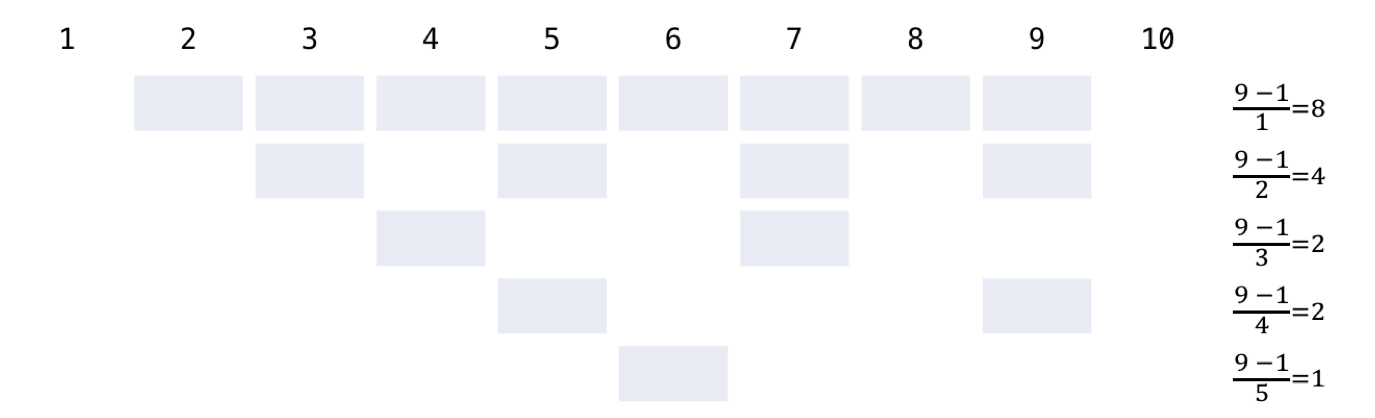
\includegraphics{../img/intervalos.png}
  \end{itemize}
\item
  Adaptando para o nosso caso e incluindo o elemento inicial, ao todo
  serão afetados\\
  \texttt{(n\ -\ 1\ -\ k*k)\ //\ (2*k)\ +\ 1} elementos, cujos valores
  devem passar para \texttt{False}.
\end{itemize}

Depois de implementar essa alteração, chegamos à nossa versão
definitiva.

    \subsubsection{Solução}\label{soluuxe7uxe3o}

    \begin{Verbatim}[commandchars=\\\{\}]
{\color{incolor}In [{\color{incolor}32}]:} \PY{k+kn}{from} \PY{n+nn}{time} \PY{k}{import} \PY{n}{perf\PYZus{}counter}
         
         \PY{n+nb}{print}\PY{p}{(}\PY{n}{f}\PY{l+s+s2}{\PYZdq{}}\PY{l+s+s2}{\PYZob{}}\PY{l+s+s2}{\PYZsq{}}\PY{l+s+s2}{n}\PY{l+s+s2}{\PYZsq{}}\PY{l+s+s2}{:\PYZgt{}8\PYZcb{}  }\PY{l+s+s2}{\PYZob{}}\PY{l+s+s2}{\PYZsq{}}\PY{l+s+s2}{demora}\PY{l+s+s2}{\PYZsq{}}\PY{l+s+s2}{:\PYZgt{}10\PYZcb{}  }\PY{l+s+s2}{\PYZob{}}\PY{l+s+s2}{\PYZsq{}}\PY{l+s+s2}{\PYZsh{}primos}\PY{l+s+s2}{\PYZsq{}}\PY{l+s+s2}{:\PYZgt{}8\PYZcb{}  }\PY{l+s+s2}{\PYZob{}}\PY{l+s+s2}{\PYZsq{}}\PY{l+s+s2}{P[:4]}\PY{l+s+s2}{\PYZsq{}}\PY{l+s+s2}{:12\PYZcb{}  }\PY{l+s+s2}{\PYZob{}}\PY{l+s+s2}{\PYZsq{}}\PY{l+s+s2}{P[\PYZhy{}4:]}\PY{l+s+s2}{\PYZsq{}}\PY{l+s+s2}{\PYZcb{}}\PY{l+s+s2}{\PYZdq{}}\PY{p}{)}
         
         \PY{k}{for} \PY{n}{n} \PY{o+ow}{in} \PY{p}{[}\PY{l+m+mi}{10}\PY{p}{,} \PY{l+m+mi}{100}\PY{p}{,} \PY{l+m+mi}{1000}\PY{p}{,} \PY{l+m+mi}{10000}\PY{p}{,} \PY{l+m+mi}{100000}\PY{p}{,} \PY{l+m+mi}{1000000}\PY{p}{]}\PY{p}{:}
                 
             \PY{n}{start} \PY{o}{=} \PY{n}{perf\PYZus{}counter}\PY{p}{(}\PY{p}{)}
             
             \PY{n}{crivo} \PY{o}{=} \PY{p}{[}\PY{k+kc}{True}\PY{p}{]} \PY{o}{*} \PY{n}{n}
             \PY{k}{for} \PY{n}{k} \PY{o+ow}{in} \PY{n+nb}{range}\PY{p}{(}\PY{l+m+mi}{3}\PY{p}{,} \PY{n+nb}{int}\PY{p}{(}\PY{n}{n}\PY{o}{*}\PY{o}{*}\PY{l+m+mf}{0.5}\PY{p}{)} \PY{o}{+} \PY{l+m+mi}{1}\PY{p}{,} \PY{l+m+mi}{2}\PY{p}{)}\PY{p}{:}
                 \PY{k}{if} \PY{n}{crivo}\PY{p}{[}\PY{n}{k}\PY{p}{]}\PY{p}{:}
                     \PY{n}{crivo}\PY{p}{[}\PY{n}{k}\PY{o}{*}\PY{n}{k}\PY{p}{:}\PY{p}{:}\PY{l+m+mi}{2}\PY{o}{*}\PY{n}{k}\PY{p}{]} \PY{o}{=} \PY{p}{[}\PY{k+kc}{False}\PY{p}{]} \PY{o}{*} \PY{p}{(}\PY{p}{(}\PY{n}{n} \PY{o}{\PYZhy{}} \PY{l+m+mi}{1} \PY{o}{\PYZhy{}} \PY{n}{k} \PY{o}{*} \PY{n}{k}\PY{p}{)} \PY{o}{/}\PY{o}{/} \PY{p}{(}\PY{l+m+mi}{2} \PY{o}{*} \PY{n}{k}\PY{p}{)} \PY{o}{+} \PY{l+m+mi}{1}\PY{p}{)}
                     
             \PY{n}{P} \PY{o}{=} \PY{p}{[}\PY{l+m+mi}{2}\PY{p}{]} \PY{o}{+} \PY{p}{[}\PY{n}{i} \PY{k}{for} \PY{n}{i} \PY{o+ow}{in} \PY{n+nb}{range}\PY{p}{(}\PY{l+m+mi}{3}\PY{p}{,} \PY{n}{n}\PY{p}{,} \PY{l+m+mi}{2}\PY{p}{)} \PY{k}{if} \PY{n}{crivo}\PY{p}{[}\PY{n}{i}\PY{p}{]}\PY{p}{]}
         
             \PY{n}{end} \PY{o}{=} \PY{n}{perf\PYZus{}counter}\PY{p}{(}\PY{p}{)}
             
             \PY{n+nb}{print}\PY{p}{(}\PY{n}{f}\PY{l+s+s1}{\PYZsq{}}\PY{l+s+si}{\PYZob{}n:8\PYZcb{}}\PY{l+s+s1}{  }\PY{l+s+s1}{\PYZob{}}\PY{l+s+s1}{end \PYZhy{} start:10.5f\PYZcb{}  }\PY{l+s+s1}{\PYZob{}}\PY{l+s+s1}{len(P):8\PYZcb{}  }\PY{l+s+si}{\PYZob{}P[:4]\PYZcb{}}\PY{l+s+s1}{  }\PY{l+s+si}{\PYZob{}P[\PYZhy{}4:]\PYZcb{}}\PY{l+s+s1}{\PYZsq{}}\PY{p}{)}
\end{Verbatim}


    \begin{Verbatim}[commandchars=\\\{\}]
       n      demora   \#primos  P[:4]         P[-4:]
      10     0.00194         4  [2, 3, 5, 7]  [2, 3, 5, 7]
     100     0.00001        25  [2, 3, 5, 7]  [79, 83, 89, 97]
    1000     0.00006       168  [2, 3, 5, 7]  [977, 983, 991, 997]
   10000     0.00034      1229  [2, 3, 5, 7]  [9941, 9949, 9967, 9973]
  100000     0.00377      9592  [2, 3, 5, 7]  [99961, 99971, 99989, 99991]
 1000000     0.04960     78498  [2, 3, 5, 7]  [999959, 999961, 999979, 999983]

    \end{Verbatim}

    E, agora, nosso algoritmo tem desempenho de gente grande...


    % Add a bibliography block to the postdoc
    
    
    
    \end{document}
